% Ejemplo del uso de latemplate para escribir tesis/memorias de la Universidad Diego Portales.
%
% Eviar bugs a: Adín Ramírez, adin.ramirez (at) mail.udp.cl

% Puede generar borradores si omite la opción "final" de la clase.
%\documentclass{udpthesis}

\PassOptionsToPackage{table}{xcolor}
\RequirePackage{xcolor} % [table] 
\documentclass[final]{udpthesis}


% Establecemos el sistema para uso del español
% Babel ya esta cargado dentro de updthesis
\usepackage[T1]{fontenc} % output
\usepackage[utf8]{inputenc}% input
\usepackage{lmodern}
\usepackage{dsfont}

\usepackage{afterpage}
\usepackage{lscape}
% Agregue aca otros packetes que le sean de utilidad
% Matemáticas
\usepackage{amsmath}

% Gráficos
\usepackage{graphicx}
% \usepackage{subfig}

% Código
% \usepackage{listings}

% Referencias
\usepackage{cite}

\usepackage{subcaption}

% Gráficos, tablas, etc.
\usepackage{pgfplots, pgfplotstable, booktabs, colortbl, siunitx, array}
\sisetup{table-auto-round}

% Establecemos el tema a utilizar. 
% Debe existir el archivo udpthesisEIT.sty en su sistema TeX para poder utilizarlo.
\udptheme{EIT}


%%%%%%%%%%%%%%%%%%%%%%%%%%%%%%%
\usepackage{xspace}
\makeatletter
\DeclareRobustCommand\onedot{\futurelet\@let@token\@onedot}
\def\@onedot{\ifx\@let@token.\else.\null\fi\xspace}

\def\eg{\emph{e.g}\onedot} \def\Eg{\emph{E.g}\onedot}
\def\ie{\emph{i.e}\onedot} \def\Ie{\emph{I.e}\onedot}
\def\cf{\emph{c.f}\onedot} \def\Cf{\emph{C.f}\onedot}
\def\etc{\emph{etc}\onedot} \def\vs{\emph{vs}\onedot}
\def\wrt{w.r.t\onedot} \def\dof{d.o.f\onedot}
\def\etal{\emph{et al}\onedot}
\def\adhoc{\emph{ad hoc}\xspace}
\makeatother

\usepackage{amsthm}
\newtheorem{definition}{Definición}[chapter]

% declare my operator
\usepackage{scalerel}
\DeclareMathOperator*{\cat}{\scalerel*{\|}{\sum}}


%%%%%%%%%%%%%%%%%%%%%%%%%%%%%%%
%\cat_{i = 1} {N}

\begin{document}
%% Inicio de la portada
\frontmatter
% Título del tema
\title{Reconocimiento de expresiones faciales en imágenes dinámicas utilizando un descriptor basado en rayos de flujo}

% El autor(es) de la tesis
\author{Miguel Antonio Rodríguez Santander}
\email{m.rodriguezs1990@gmail.com-}% utilice un correo que revise después de graduado
% o una lista de autores
%\author{Juan Bar\\José Foo}

% Fecha a aparecer en la tesis
\date{Diciembre, 2014}

% Profesor guía
\professor{Adín Ramírez}
% Comité evaluador
% puede tener uno o dos evaluadoers (deje en blanco el parámetro que no utilizará)
\committee{ David Röthlisberger }{ Andrea Nieto }
% \committee{Nicola Tesla}{Isaac Newton}

% Dedicatoria
\dedicatory{\textit{``Violence is the last refuge of the incompetent.''} - Isaac Asimov.}
%
% Agradecimientos
\acknowledgment{Agradezco a mi familia por ser fuente de apoyo constante e incondicional en toda mi vida y más aún en mis duros años de estudio.
A mi profesor guía Adín Ramírez por la motivación de siempre estar educándome para ser un mejor profesional y por su paciencia.
A mis amigos por apoyarme incondicionalmente en mis aventuras y desventuras, especialmente a Felipe Troncoso, Rodrigo Fuenzalida y Camilo Contreras quienes ayudaron al desarrollo de esta tesis.}

% Generamos la portada
\makecover

% Indices y listas
\tableofcontents% tabla de contenido
\listoffigures%   índice de figuras
\listoftables%    índice de tablas
% puede agregar otras listas o índices acá de ser necesario

% Abstrac en inglés
\begin{abstract}
Facial expression recognition is an area of research in constant growth, due to the large number of new technologies that have recently been developed. Current technological advances in this area allow us to create or enhance human-computer interfaces, which helps improve the quality of life of people that use such devices. Applications in areas such as medicine, marketing, psychology, robotics, public safety, among others, generate a high demand for this kind of technologies.

This thesis propose a novel space-temporal descriptor for the recognition of the six universal facial expressions (Joy, Disgust, Anger, Fear, Sadness and Surprise). We introduce a new term called ray flux, which consist in the codification of videos using relevant human facial movements. The creation of this new descriptor has four stages: Database preprocessing, this step entails the applications of face recognition and motion correction techniques;  Micro-descriptors extraction, stage where the ray flux extraction occurs, which is applied over every frame of the video; Creating macro-descriptors, we then proceeds to create the descriptors for each individual video, using techniques such as Bag of Visual Words and Clustering; Training and classification, in this final step we output a model, by feeding the already proccesed data to the Support Vector Machines, this model is then used to classify the system entries.

In general we manage to obtain 44\% accuracy where the state of the art methods achieve 88\% accuracy for the same input data, instead of focusing our work on the accuracy obtained, we present new techniques and methods that we believe have a lot of new potential applications.


\end{abstract}

% Resumen
\begin{resumen}
El reconocimiento de expresiones faciales es un área de investigación en constante crecimiento, debido a la gran cantidad de nuevas tecnologías que se pueden desarrollar. Los actuales avances tecnológicos en esta área permiten crear o mejorar interfaces humano-computador, las cuales ayudan a la mejor calidad de vida de las personas. Aplicaciones en áreas como la medicina, el marketing, la psicología, la robótica, seguridad pública entre otras, tienen una alta demanda de tecnologías de este estilo.

En esta tesis se propone un nuevo descriptor espacio-temporal para el reconocimiento de las seis expresiones universales (Alegría, Asco, Ira, Miedo Sorpresa y Tristeza), para el cual se introduce un nuevo término llamado \textit{Rayo de flujo}, el cual consiste en una nueva codificación  basada en el movimiento de las áreas importantes del rostro humano a través de los cuadros del vídeo analizado. La creación de este nuevo descriptor consta de cuatro etapas:  \emph{Preprocesamiento de la base de datos}, la cual consiste en aplicar técnicas de reconocimiento de rostro y corrección de movimiento sobre los datos de entrada. \emph{Extracción de micro-descriptores}, etapa en la cual se realiza el proceso de extracción de \textit{rayos de flujo} sobre todos los cuadros del vídeo. \emph{Creación de macro-descriptores}, luego de la extracción de micro-descriptores se procede a crear los descriptores generales de cada vídeo, utilizando técnicas como \textit{Bag of Words} y \textit{Clustering}. Y por último \emph{Entrenamiento y clasificación}, etapa en la cual se entrena el modelo utilizando  las \emph{Support Vector Machines}, para luego utilizar este modelo en la clasificación de las nuevas entradas. En general los resultados obtenidos por nuestro método no superan el 48\% de \textit{Accuracy}, lo cual es un resultado pobre al ser comparado con métodos del estado del arte, los cuales obtienen valores superiores al 88\%. Por esto proponemos realizar mejoras en la etapa de extracción de \textit{rayos}, tales como solo utilizar la componente vertical de los movimientos o a su vez utilizar el angulo de movimiento para la creación de los \textit{rayos}, ademas también proponemos realizar una segmentación de las regiones importantes del rostro (ojos, nariz y boca), a las cuales se realiza todo el procesamiento del algoritmo.
\end{resumen}



% Inicio del contenido
\mainmatter

% Capítulos y secciones del documento
% Aca se incluyen los archivos con el texto de los capitulos
% Incluyo el archivo cap-intro.tex
\chapter[Introducción]{Introducción}
\label{ch:intro}

\section{Motivación}
\label{sec:motivacion}
Con los actuales avances tecnológicos, el reconocimiento de expresiones faciales (FER, Facial Expression Recognition) forma parte importante de una rama de la inteligencia artificial, específicamente el reconocimiento de patrones.  Las investigaciones sobre el FER permiten el desarrollo de futuras tecnologías ligadas al desarrollo de interfaces centradas en el humano. 

Existen diversas aplicaciones tecnológicas enfocadas al reconocimiento de expresiones faciales aplicadas en distintas áreas del conocimiento humano, tales como:  la medicina, que se utiliza para la detección de enfermedades y rehabilitación de trastornos mentales; la psicología, para reportes sobre estados de ánimo; el marketing, la posibilidad de una segmentación del cliente al cual se quiere llegar con la publicidad; la robótica, la interacción humano-robot; la seguridad, para combatir fraudes de pasaportes, soporte al orden público e identificación de personas desaparecidas; entre otras áreas.

Diversas empresas también han utilizado estos avances de reconocimiento facial como un componente que aporta información en las tecnologías que ofrecen. Un ejemplo de esto es  Google que utiliza el FER en su motor de búsqueda de imágenes y se proyecta utilizar este reconocimiento para aportar información a la entrada de video de los Google Glass~\cite{GoogleGlass}. Otro ejemplo es Facebook que usa la detección de rostros en  fotos para realizar el etiquetado rápido de usuarios.

Los estudios de Mehrabian~\cite{Mehrabian1968} sobre la comunicación oral indican que las expresiones faciales contribuyen con aproximadamente el 55\% de la transmisión del mensaje, lo cual es un valor mucho mayor que la parte verbal con 7\% y la parte vocal un 38\%.

El objetivo de este proyecto es buscar un nuevo descriptor espacio temporal para reconocer expresiones faciales. Para esto se propone un nuevo método utilizando imágenes dinámicas, el cual utilizaremos para reconocer las seis expresiones faciales universales: alegría, asco, ira, miedo, sorpresa y tristeza.

\section{Problema}
\label{sec:problema}

En la actualidad existen muchos métodos que permiten resolver el problema del reconocimiento de expresiones faciales, algunos utilizan el sistema de codificación de acciones faciales (FACS) creado por Ekman~y~Friesen~\cite{Ekman1978}, entre los cuales están las investigaciones de Pantic y Rothkrantz~\cite{Pantic2004}, Lien et al.~\cite{Lien1998}, Pantic y Patras~\cite{Pantic2006}, entre otros. Otras investigaciones utilizan métodos de reconocimiento basados en características geométricas o de apariencia, entre los cuales están Ramírez et al.~\cite{RamirezRivera2013}, utilizando Local Direccional Number Patterns; Lyons et al.~\cite{Lyons1998}, utilizando filtros de Gabor; Ahonen et al.~\cite{Ahonen2006}, utilizando Local Binary Patterns (LBP por sus siglas en inglés).

Las últimas investigaciones se centran en poder resolver el problema del reconocimiento de expresiones agregando la variable temporal $t$, la cual indica que ya no solo se quiere reconocer en imágenes sino que en secuencias de imágenes o videos, con lo cual además de necesitar crear algoritmos que permitan buscar la expresión a través del tiempo, también deben ser algoritmos eficientes, debido a la gran cantidad de cálculos que se deben realizar. Existen distintas investigaciones que intentan resolver el problema del reconocimiento en vídeos: Zhao y Pietikäinen~\cite{Zhao2006}, crean una nueva codificación basada en LBP introduciendo la variable del tiempo, esta codificación recibe el nombre de Volume Local Binary Patterns; Zhao y Pietikäinen~\cite{Zhao2006}, también crean otra codificación basada en LBP en la cual utilizan tres planos ortogonales, llamada LBP-TOP; Buenaposada~\etal~\cite{Buenaposada2008}, estiman la deformación de los componentes no rígidos del rostro; Yeasin~\etal~\cite{Yeasin2004}, crean una firma temporal de cada entrada, con la cual entrenan sus modelos; Xiang~\etal~\cite{Xiang2008}, utilizan la transformada de Fourier para realizar la extracción de características, y luego utilizan Fuzzy C-means para generar los modelos.

En este trabajo proponemos un nuevo método que nos permita poder resolver el problema del reconocimiento de expresiones faciales en videos. La idea general de nuestra solución es juntar métodos de distintas áreas de las ciencias de la computación y crear una nueva forma de representar las expresiones faciales en video. En general introducimos un nuevo micro-descriptor que llamamos \textit{rayo de flujo}, el cual junto con técnicas de aprendizaje maquina (machine learning, en inglés), recuperación de información (information retrieval, en inglés), visión por computador (computer vision, en inglés) y reconocimiento de patrones (pattern recognition, en inglés), nos permitirán crear un modelo que realice el reconocimiento de las seis expresiones faciales universales. 

 %ésta debe ser una solución robusta, puesto que es necesario poder lograr resultados comparables con los actuales métodos ya creados. Esta solución debe poder responder preguntas como ¿Es posible crear un modelo de clasificación a partir de las teorías propuestas en este trabajo?, de ser así, ¿Qué tan buena es la representación creada por el modelo?, ¿Cómo se compara con los algoritmos que ya resuelven este problema?, ¿Qué tan eficiente es con respecto al tiempo de ejecución es el algoritmo?, ¿Es posible implementar esta idea para reconocimiento en tiempo real?, \etc.



\section{Solución propuesta}
\label{sec:solucion}

Para este nuevo método se introduce un nuevo micro-descriptor, el cual nos permite realizar el seguimiento de las regiones de interés (ROI, regions of interest) que denominaremos \textit{rayo de flujo} o simplemente \textit{rayo}.


\subsection{Pipeline}

La cadena de procedimientos ordenados o \textit{pipeline} de este método se divide en cuatro grandes etapas: preprocesamiento de la base de datos, extracción de micro-descriptores, creación de macro-descriptores, y entrenamiento y clasificación, este procedimiento puede ser visto en la Figura~\ref{intro:fig:pipeline}.
	\begin{figure}[b]
		\centering
		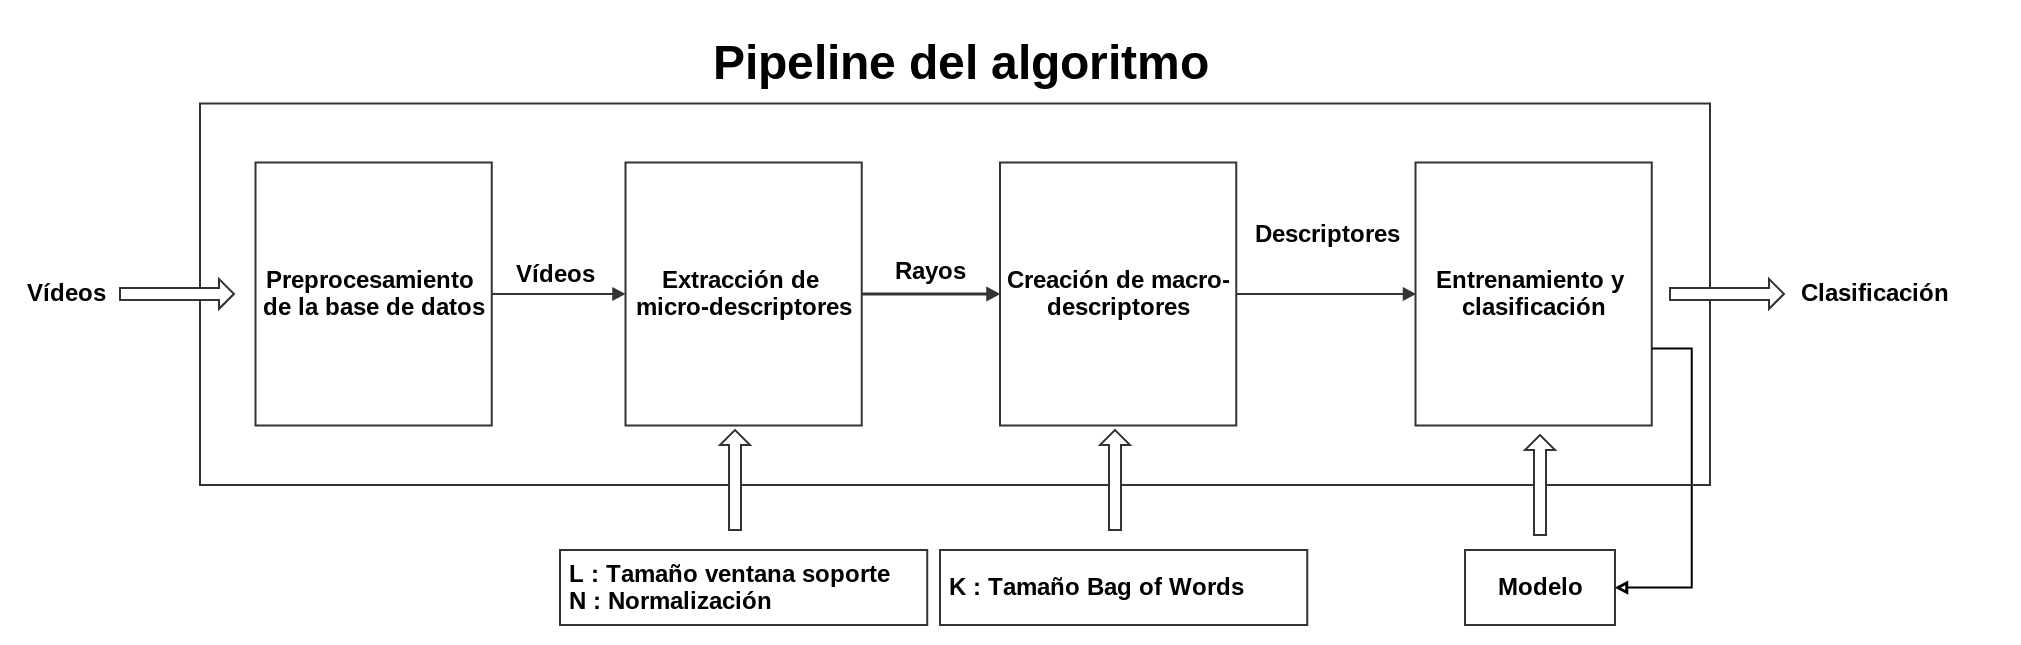
\includegraphics[width=1\textwidth]{Figuras/Diagramas/pipeline.png}
		\caption{Pipeline del algoritmo propuesto.}
		\label{intro:fig:pipeline}
	\end{figure}		
	
\textbf{Preprocesamiento de la base de datos.}
Antes de poder realizar la extracción de características de los videos, es necesario realizar un preprocesamiento sobre éstos, esto debido a que los videos pueden tener ciertos elementos que estropean la extracción de características. Para evitar agregar ruido al video se utilizan dos técnicas que permiten obtener solo el rostro de la persona a representar su expresión y a su vez corregir los movimientos que éstos puedan tener. Esta etapa será profundizada en la Sección~\ref{sec:proc_bdd}.


\textbf{Extracción de micro-descriptores.}
Este proceso consiste en la extracción de los rayos de flujo de cada uno de los videos preprocesados, para esto, primero se seleccionan las regiones de interés de la cara. Luego, para cada uno de los pixeles de la región, se procede a calcular el movimiento de este píxel con respecto al cuadro siguiente, y así sucesivamente con cada uno de los cuadros del vídeo. Luego de calcular el movimiento para cada píxel en cada cuadro, se obtiene el conjunto de \textit{rayos} o micro-descriptores que definen el video. Esta etapa será profundizada en la Sección~\ref{sec:micro_descriptores}.


\textbf{Creación de macro-descriptores.}
Luego de extraer cada uno de los micro-descriptores, se procede a crear utilizar la técnica de la bolsa de palabras visuales (\textit{Bag of Visual Words} en inglés), este método es utilizado para poder agrupar los \textit{rayos} en $k$ grupos, los cuales definen el espacio de los macro-descriptores. Cada \textit{rayo} extraído de los vídeos pertenece únicamente a un solo grupo, por lo tanto es posible para cada vídeo obtener un histograma de la frecuencia de aparición de cada uno de estos grupos en sus \textit{rayos}. Este histograma obtenido es el macro-descriptor que se utiliza para poder entrenar y clasificar. Esta etapa será profundizada en la Sección~\ref{sec:macro-descriptores}.


\textbf{Entrenamiento y clasificación.}
Luego de obtener los macro-des\-crip\-tores para cada uno de los vídeos, se procede a la etapa de entrenamiento y posterior clasificación. Para poder entrenar y clasificar con los macro-descriptores obtenidos en la etapa anterior, se utilizan las Maquinas de Vectores de Soporte (Support Vector Machines por sus siglas en ingles). Esta técnica permite dividir el espacio vectorial representado por los descriptores de entrenamiento, para luego ser probado por los descriptores que se obtienen en la clasificación o prueba del modelo creado. Para poder probar la efectividad de la clasificación se utiliza la técnica de validación cruzada, la cual permite realizar distintas pruebas de entrenamiento y clasificación, para obtener cual es el porcentaje de efectividad del método. Esta etapa será profundizada en la Sección~\ref{sec:clasificacion}.

\subsection{Ventajas potenciales del método}
En esta investigación se introduce un nuevo micro-descriptor llamado \textit{Rayo de flujo}, en simples palabras, 
un \textit{rayo de flujo} es el conjunto de variaciones que tiene un píxel determinado a lo largo del vídeo, esto será explicado en mayor profundidad en la Sección~\ref{sec:micro_descriptores}.

Éste, al ser un enfoque nuevo no visto en otras investigaciones, las distintas ventajas potenciales serán evaluadas a lo largo de la investigación, en general nos centraremos en demostrar o desmentir las siguientes incógnitas:

\begin{itemize}
	\item ¿Permitirán los \textit{rayos} solucionar el problema de la variable temporal?
	\item Al ser un modelado espacio-temporal de los píxeles, los \textit{rayos}, ¿permitirán ver cual es el comportamiento de los pixeles a través del tiempo?
	\item ¿Permitirán los \textit{rayos} modelar micro-patrones en los movimientos del rostro que no pueden ser vistos a simple vista por los humanos?, de ser cierto, ¿estos micro-patrones aportarán mayor información al modelo de clasificación?.
	\item ¿Existe la posibilidad de que cada una de las expresiones faciales universales pueda tener asociado un conjunto de \textit{rayos} que la definan?. 
\end{itemize}


\section{Objetivos}
\label{subsec:objetivos}
A continuación se describen los objetivos de este trabajo:

\subsection{Objetivo general}
\label{subsubsec:objgeneral}
Crear un descriptor espacio-temporal basado en el seguimiento del movimiento de los pixeles para el reconocimiento de expresiones faciales en video.

%Crear un descriptor para el reconocimiento de expresiones faciales en vídeo utilizando micro patrones basados en el seguimiento del flujo de los movimientos del rostro.
%\item Crear o encontrar una métrica que permita la comparación entre rayos luego del proceso de normalización.
%\item Evaluar y comparar el método creado con el estado del arte hasta antes de comenzar la memoria. 
%\item Definir un método de elección de las regiones de interés del rostro.
%\item Definir un método de elección de las regiones de interés del rostro.

\subsection{Objetivos específicos}
\label{subsubsec:objgeneral}
	\begin{enumerate}
		\item Modelar el comportamiento de los pixeles a través del tiempo.
		\item Definir una codificación que permita la normalización de los rayos de flujo.
		\item Estudiar la distribución de los movimientos de los pixeles sobre el rostro.
	\end{enumerate}
% Incluyo el archivo cap-tema.tex
\chapter[Estado del arte]{Estado del arte}
\label{ch:estado_del_arte}

\chapter[Algoritmo propuesto]{Algoritmo propuesto}
\label{ch:algoritmo}
\section{Pipeline}
\label{sec:pipeline}
Para poder solucionar el problema propuesto en la Sección~\ref{sec:problema}, se propone un algoritmo compuesto por cuatro módulos. \emph{Preprocesamiento de la base de datos}, módulo encargado de quitar todo el ruido de los vídeos de entrenamiento, \emph{extracción de micro-descriptores}, encargado de dividir el vídeo en distintas regiones de interés para crear un micro-descriptor basado en el movimiento interno de éstas, \emph{creación de macro-descriptores}, toma los micro-descriptores y crea un nuevo macro-descriptor por vídeo utilizando técnicas de \textit{clustering}, y por último \emph{entrenamiento y clasificación}, encargado de crear un modelo de clasificación con los descriptores de entrenamiento, para luego utilizar este modelo para la posterior clasificación de nuevos vídeos. Presentamos este modelo en la Figura~\ref{algoritmo:fig:pipeline}.

	\begin{figure}[bt]
		\centering
    		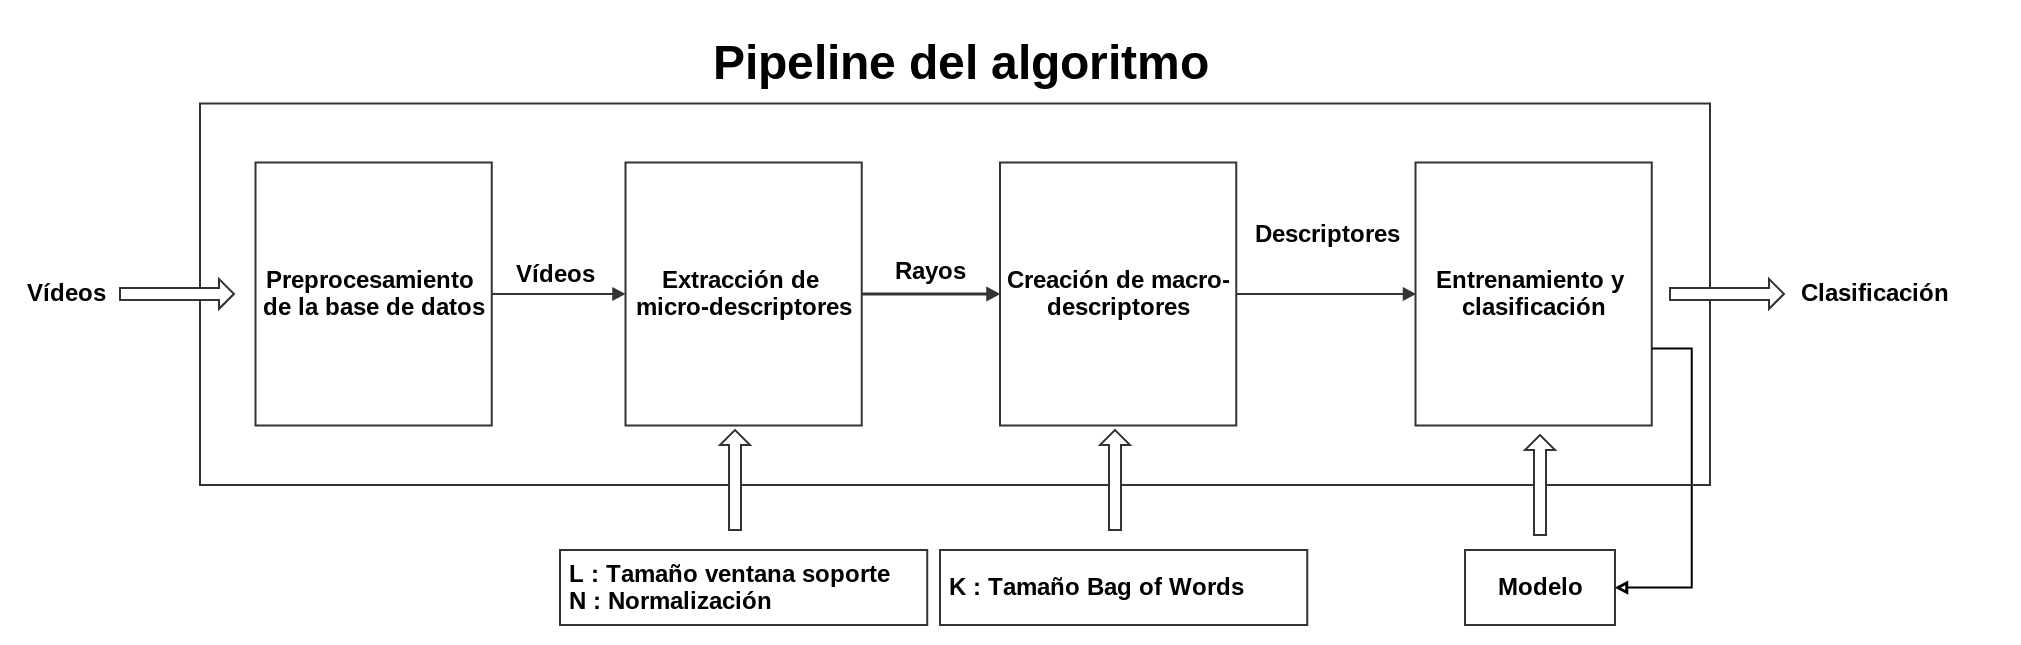
\includegraphics[width=1\textwidth]{Figuras/Diagramas/pipeline.png}
  		\caption{Pipeline del algoritmo propuesto.}
  		\label{algoritmo:fig:pipeline}
	\end{figure}	


\section{Preprocesamiento de la base de datos}
\label{sec:proc_bdd}
	El preprocesamiento de la base de datos es la etapa donde se realiza la limpieza de todos los datos que entran al algoritmo. Cada uno de los vídeos de entrada tienen elementos que no aportan mayor información al método, sino que también pueden aportar ruido, de tal manera se procede a eliminar todos estos elementos. Este procedimiento se divide en dos etapas: \emph{cetección de rostros}, que utiliza el algoritmo de Viola-Jones para encontrar el rostro del primer cuadro, y el segundo \emph{corrección de movimiento}, que utiliza el cuadro encontrado del rostro para corregir el movimiento de todos los cuadros del vídeo. Este procedimiento puede ser visualizado en la Figura~\ref{algoritmo:fig:preprocesamiento}. 
	
	\begin{figure}[tb]
		\centering
    		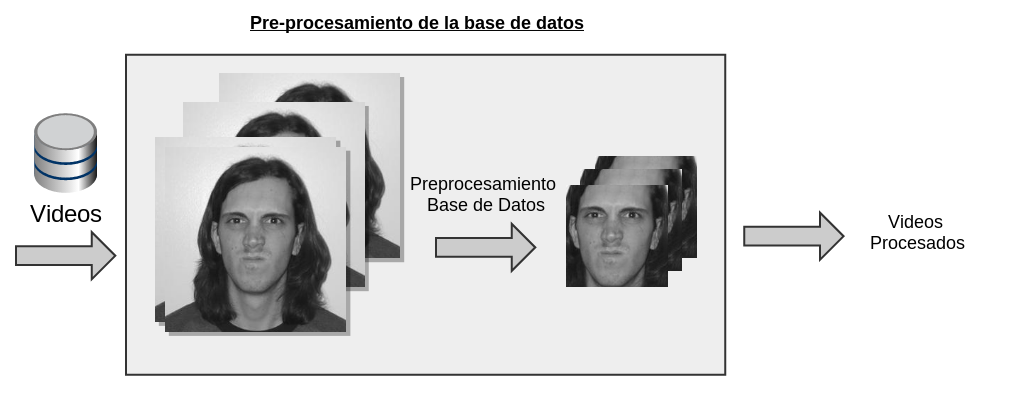
\includegraphics[width=1\textwidth]{Figuras/Diagramas/Preprocesamiento.png}
  		\caption{Diagrama del preprocesamiento de los datos.}
  		\label{algoritmo:fig:preprocesamiento}
	\end{figure}	

	
	\subsection{Detección de rostros}
	\label{algoritmo:det_rostro}
	Para cada uno de los vídeos que se utilizarán en el algoritmo es necesario quitar todos los elementos que no aportan información. De tal forma, utilizamos un algoritmo de detección de rostros, el cual obtiene los vértices del rectángulo que encierra la cara en el primer cuadro. Utilizaremos este rectángulo en la fase de corrección de movimiento del rostro. 
		
	\subsection{Corrección de movimiento}
	\label{algoritmo:cor_movimiento}
	Luego de realizar la detección de rostros para cada uno de los cuadros del vídeo, se procede a realizar la corrección del movimiento rígida. Ésta consiste en realizar operaciones de translación y rotación sobre cada uno de los cuadros del vídeo utilizando la imagen del rostro detectado en el primer cuadro como modelo para ajustar los cuadros siguientes.


\section{Extracción de micro-descriptores}
\label{sec:micro_descriptores}
	El proceso de extracción de micro-descriptores es el núcleo del algoritmo. Este proceso es el encargado de la extracción de características directas del vídeo o imagen dinámica. Para esto se introduce un nuevo término que es denominado \textit{Rayo de flujo} o simplemente \textit{Rayo}. Éste define el movimiento de los píxeles dentro las regiones de interés (ROI por sus siglas en inglés) en los cuadros del vídeo. Esta etapa se puede dividir en tres grandes bloques, primero, la \emph{codificación}, etapa en la cual el vídeo puede ser codificado utilizando técnicas como LBP o LDN\@. Esta etapa es opcional y sera mayormente profundizada en el Capítulo~\ref{ch:exp_result}. Segundo, \emph{extracción de rayos}, la cual consiste en determinar las regiones de interés de donde se extraerán los \textit{Rayos de flujo}, y su extracción como tal. Y por ultimo, \emph{normalización}, esta etapa se encarga de llevar todos los \textit{Rayos} al mismo espacio vectorial, dado un tamaño fijo. Un diagrama de la extracción de micro-descriptores puede ser visto en la Figura~\ref{algoritmo:fig:micro_descriptores}.

\afterpage{% corrige el breakpage
\begin{landscape}
	\begin{figure}[t]
		\centering
    		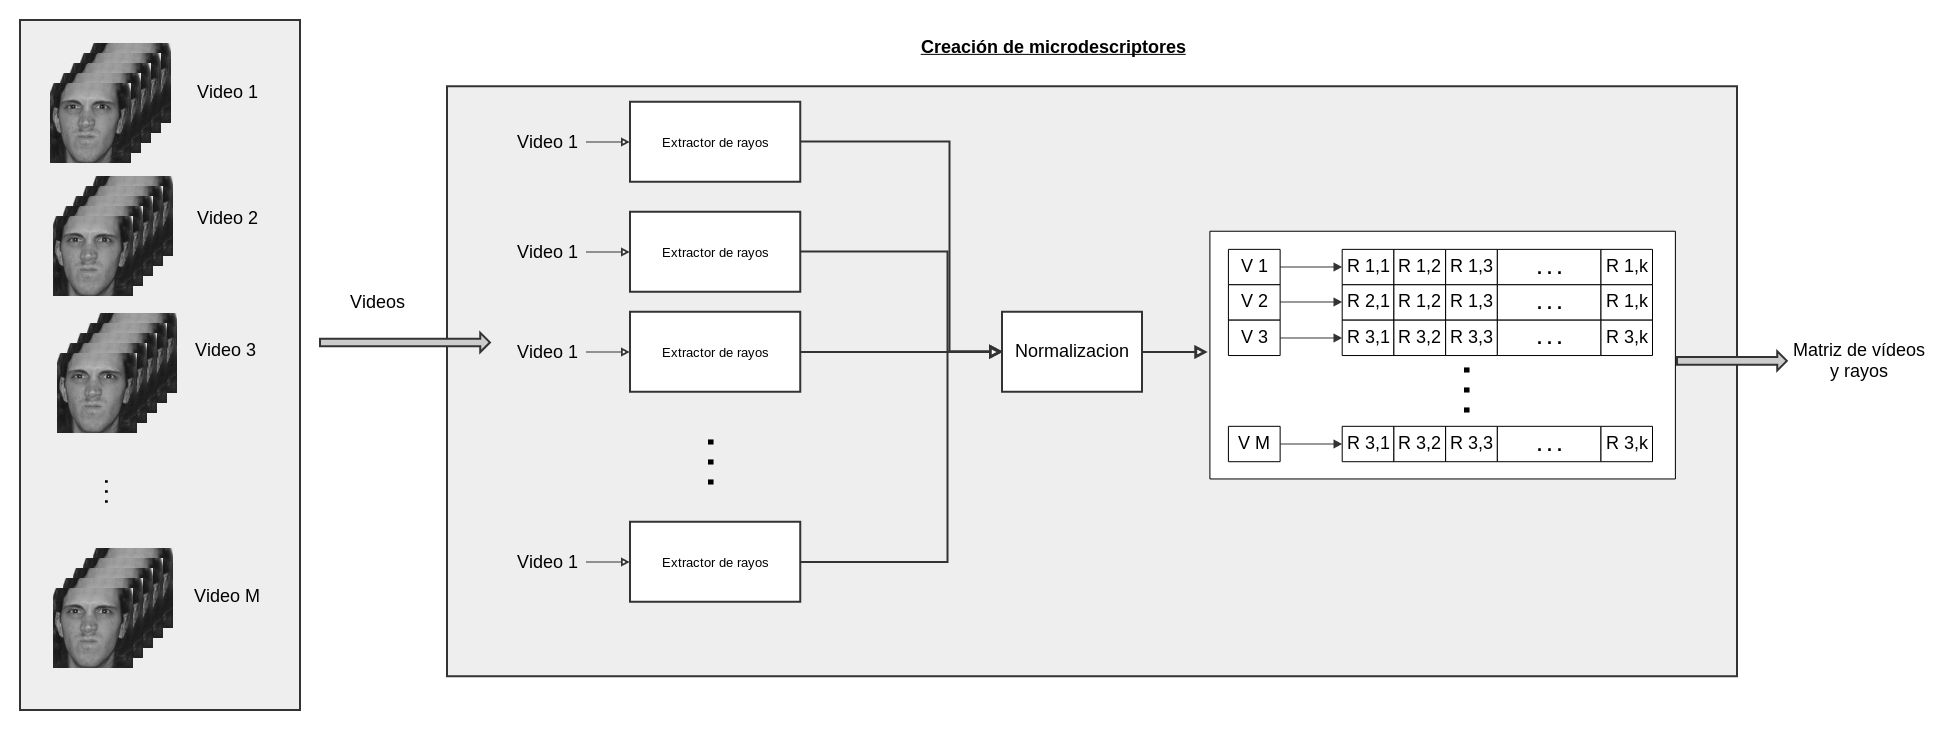
\includegraphics[width=\linewidth]{Figuras/Diagramas/Extractor_microdescriptores}
  		\caption{Diagrama general del proceso de extracción de micro-des\-crip\-to\-res.}
  		\label{algoritmo:fig:micro_descriptores}
	\end{figure}	
\end{landscape}}

	\subsection{Elección de regiones de interés}
	\label{algoritmo:elecc_roi}
	De cada vídeos que se quiere procesar, después de realizar el preprocesamiento definido en la Sección~\ref{sec:proc_bdd}, se seleccionan las regiones de interés a las cuales se les extraerá los \textit{Rayos}. Las áreas se seleccionarán utilizando distintos criterios [$\mathds{R}(\cdot)$, ver (\ref{algoritmo:eq:roi})], por ejemplo, pueden utilizarse áreas puntuales con alta expresividad (\eg, los ojos, la boca, la nariz, \etc), o bien áreas generales (\eg, todo el rostro).
	
	De tal forma, definimos un vídeo como 
	\begin{equation}\label{algoritmo:eq:video}		
		V = \{\text{ROI}_i | 1 \leq i \le I\}, 
	\end{equation}
	donde $I$ es el número de regiones de interés en el vídeo. Y además, definimos el $i$-ésimo ROI, $\text{ROI}_i^t$, como el conjunto de píxeles $(x,y)$ para un determinado cuadro $t$, tal que
	\begin{equation}\label{algoritmo:eq:roi}
		\text{ROI}_{i}^{t} = \{(x,y) | (x,y,t) \in \mathds{R}(i)\},
	\end{equation}
	donde $\mathds{R}(i)$, es una función que devuelve la $i$-ésima región en que dividimos el vídeo, según el criterio antes mencionado.

	\subsection{Extracción de rayos}
	\label{algoritmo:ext_rayos}
	
	Para esta sección se introducen dos términos nuevos: la \textit{región de soporte} y la \textit{ventana de búsqueda}. La \textit{región de soporte} es utilizada para calcular el movimiento del píxel central con respecto al cuadro siguiente. Similarmente, la \textit{ventana de búsqueda} es el espacio supuesto en el cual se pudo haber desplazado la región de soporte en el siguiente cuadro, y por ende, donde lo buscaremos. Definimos estos términos formalmente a continuación.
	
	\begin{definition}[Región de soporte]	
  Dado un píxel $(x,y)$ en un cuadro $t$, definimos una región de soporte RS, de tamaño $R \times R$ (donde $R$ es impar), como la subregión del cuadro $t$ que está centrada en el píxel $(x,y)$.
	\end{definition}

	\begin{definition}[Ventana de búsqueda]
	Dado un píxel $(x,y)$ en un cuadro $t$, definimos la ventana de búsqueda WS, de  tamaño $W \times W$(donde $W < R$ y $W$ es impar), como la subregión del cuadro $t+1$ que está centrada en el píxel $(x,y)$.
	\end{definition}
		
	Dado un píxel $(x,y)$ en el cuadro $t$, la extracción de rayos consiste en obtener una \textit{región de soporte}, $\text{RS}(x,y,t)$, una \textit{ventana de búsqueda}, $\text{WS}(x,y,t)$, y encontrar la posición de mejor emparejamiento entre la \textit{región de soporte} y la \textit{ventana de búsqueda}. Esta búsqueda se realiza calculando el error Cuadrático Medio (MSE por sus siglas en inglés), \begin{equation}\label{algoritmo:eq:mse}	
			\text{MSE}(\text{RS}, \text{RS}') = \sum_{x=1}^{R} \sum_{y=1}^{R} \left(\text{RS}(x,y,t) - \text{RS}'(x',y', t+1)\right)^2,
		\end{equation} 
	donde $\text{RS} = \text{RS}(x,y,t)$ es la \textit{región de soporte} del píxel $(x,y)$ en el cuadro $t$, al que esta extrayendo el \textit{rayo}, y $\text{RS}' = \text{RS}'(x',y',t+1) \in \text{WS}(x,y,t)$ es una subregión de la \textit{ventana de búsqueda} del píxel $(x,y)$ en el cuadro $t+1$ de tamaño $L$ (note que la \textit{ventana de búsqueda} del píxel $(x,y)$ en el cuadro $t$ está definida en el cuadro $t+1$).
		
	Esta operación se realiza para cada uno de los desplazamientos que puedan ser realizados por la \textit{región de soporte} dentro de la \textit{ventana de búsqueda}. De tal forma que buscamos la posición de la región $\text{RS}'$ que minimiza el MSE respecto de la \textit{región de soporte} del píxel $(x,y)$ en el cuadro $t$, $\text{RS}(x,y,t)$, de tal forma que la región $\text{RS}'$ óptima será
	\begin{equation}
		\text{RS}^* = \arg \min_{\text{RS}'}\{\text{MSE}(\text{RS},\text{RS}') | \text{RS}' \in \text{WS} \},
	\end{equation}		
	 la cual será la región $\text{RS}'$ donde el error sea mínimo, con lo que se puede deducir que la región $\text{RS}$ se desplazó a la región $\text{RS}^*$ en el tiempo $t+1$. Mediante esto se obtiene el píxel $(x^*,y^*)$ que corresponde al centro de la ventana obtenida en el proceso anterior, $\text{RS}^*$.
	
	Para calcular el desplazamiento en el cuadro $t$ de $(x,y)$ a $(x^*,y^*)$, se procede a realizar la resta de los ejes. De tal forma que
	\begin{align}
		\Delta x^{t} &= x^*-x,\\ 
		\Delta y^{t} &= y^*-y,
	\end{align}
		donde $ \Delta x^t$ y $ \Delta y^t$ son componentes del \textit{Rayo de soporte}. Definimos un \textit{Rayo de soporte} como:
	
	\begin{definition}[Rayo de soporte]
		Dado un par ordenado $(x,y)$ en el tiempo $t$, el \textit{Rayo de soporte} para dicho píxel esta definido por el nuevo par ordenado $(\Delta x^{t}, \Delta y^{t})$, de tal forma que,
		\begin{equation}
			\rho_{(x,y)} = \{(\Delta x^{t}, \Delta y^{t})~| \forall t\}.
		\end{equation}		
	\end{definition}	
		
	Los \textit{Rayos de soporte} son la estructura básica de los \textit{Rayos de flujo}, dado que al juntar todos los desplazamientos del píxel $(x,y)$ a lo largo de los cuadros del vídeo, se obtiene un conjunto de variaciones de movimientos. En palabras más formales, se define:
	
	\begin{definition}[Rayo de flujo]	
		Es el conjunto de \textit{Rayos de soporte} que representan el movimiento del píxel $(x,y)$ en cada uno de los cuadros $t$, este conjunto es definido como \textit{Rayo de flujo} o micro-descriptor, de tal forma que,
			\begin{equation}
				R(x,y)	 = \{\rho_{(x,y)}, \rho_{(x^*,y^*)}, \rho_{(x^{**},y^{**})}, ... \},
			\end{equation}
		donde ($x^{**}$,$y^{**}$) es el píxel al cual se desplazo ($x^{*}$,$y^{*}$) en el cuadro $t+2$. El desplazamiento de los \textit{rayos} puede ser visto en la Figura~\ref{algoritmo:fig:extraccion}.
	\end{definition}
	
	\begin{figure}[bt]
		\centering
    		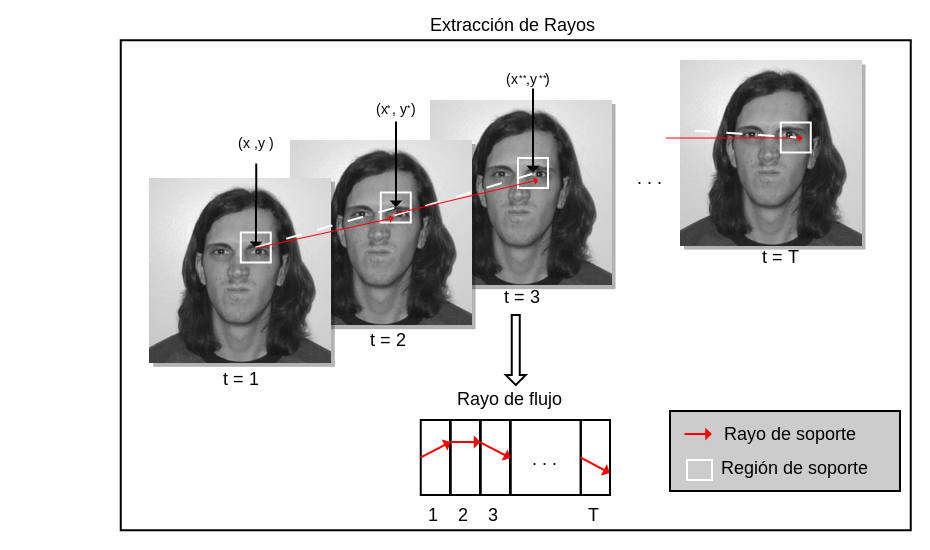
\includegraphics[width=1\textwidth]{Figuras/Diagramas/Extraccion_de_rayos.png}
  		\caption{Representación de la extracción de rayos de un vídeo.}
  		\label{algoritmo:fig:extraccion}
	\end{figure}	

	
		
		
	\subsection{Normalización de rayos}
	\label{algoritmo:normalizacion}
	Luego de obtener el total de micro-descriptores es necesario poder llevar todos los \textit{rayos} al mismo espacio vectorial, esto debido a que el tamaño de cada conjunto depende de la cantidad de cuadros $T$ del vídeo. Para este proceso se introduce una variable muy importante para el algoritmo llamada $N$, esta sera la encargada de comandar el proceso de normalización, de tal forma que se obtiene una razón de normalización
	\begin{equation}
		Rn = \frac{T}{N},
	\end{equation}
	está permite relacionar la cantidad de \textit{Rayos de soporte} $\rho$ del \textit{Rayo} $R(x,y)$ original que formaran parte de los $\rho'$ de $R(x,y)'$ normalizado. Este proceso puede ser visualizado en la Figura~\ref{algoritmo:fig:normalizacion}.
	
	\begin{figure}[bt]
		\centering
    		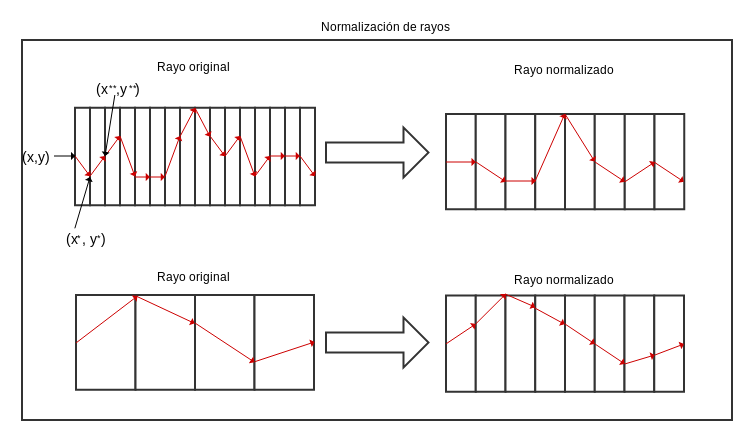
\includegraphics[width=1\textwidth]{Figuras/Diagramas/normalizacion_de_rayos.png}
  		\caption{Normalización de rayos.}
  		\label{algoritmo:fig:normalizacion}
	\end{figure}	

	
\newpage	
\section{Creación de macro-descriptores}
\label{sec:macro-descriptores}
El proceso de creación de macro-descriptores es el proceso final de la extracción de características de los vídeos. Luego de obtener un extenso conjunto de \textit{Rayos} para cada uno de los vídeos, es necesario poder crear grupos de \textit{Rayos}, los cuales puedan representar de mejor manera el espacio ya normalizado. Para esto se utilizan técnicas de \textit{clustering}. El proceso de creación de macro-descriptores puede ser visto en las Figuras~\ref{algoritmo:fig:macro_descriptores:entrenamiento} y~\ref{algoritmo:fig:macro_descriptores:clasificacion}

	\begin{figure}[bt]
		\centering
    		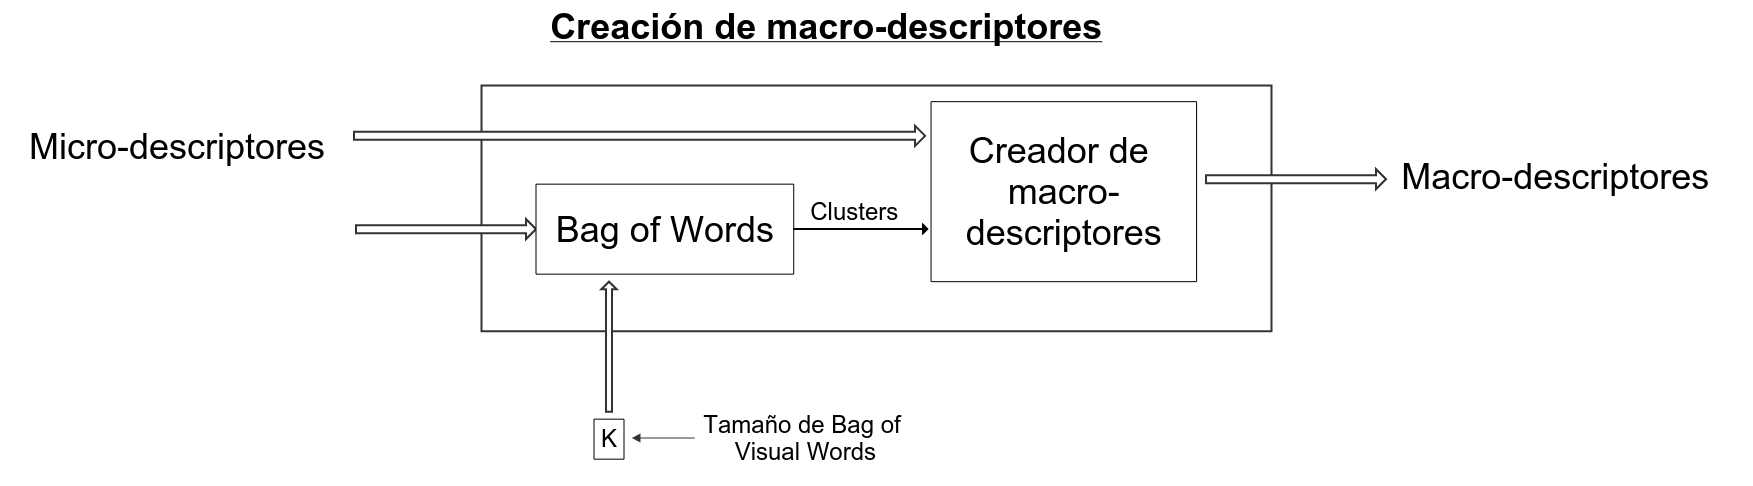
\includegraphics[width=1\textwidth]{Figuras/Diagramas/Extractor_macrodescriptores_entrenamiento.png}
  		\caption{Proceso de creación de macro-descriptores en la fase de entrenamiento.}
  		\label{algoritmo:fig:macro_descriptores:entrenamiento}
	\end{figure}	
	
	
	\begin{figure}[bt]
		\centering
    		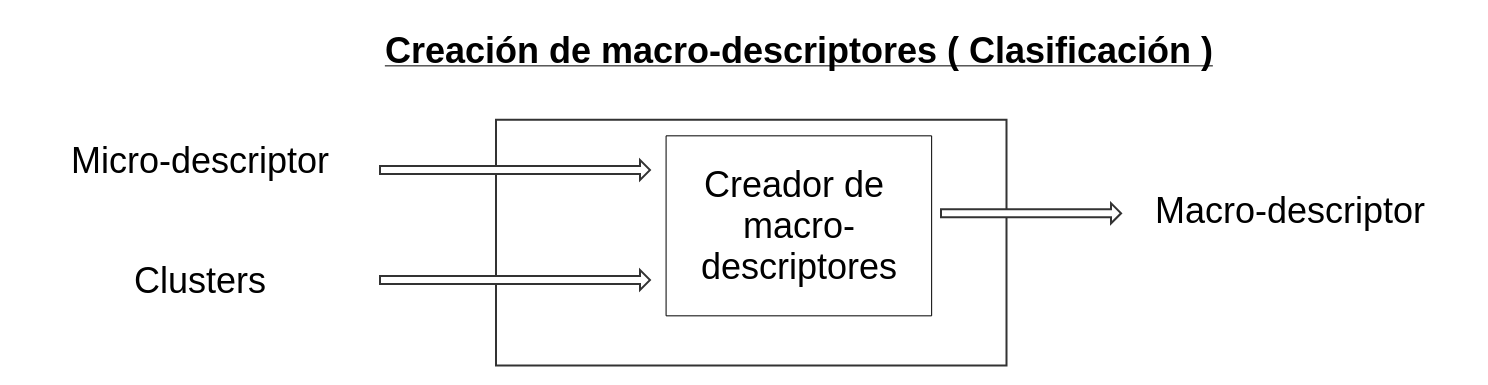
\includegraphics[width=1\textwidth]{Figuras/Diagramas/Extractor_macrodescriptores_clasificacion.png}
  		\caption{Proceso de creación de macro-descriptores en la fase de clasificación.}
  		\label{algoritmo:fig:macro_descriptores:clasificacion}
	\end{figure}	



	\subsection{Bag of Visual Words}
	\label{algoritmo:bow}
		Esta es una técnica dependiente de la cantidad $K$ de palabras que se introduzcan a la bolsa. Como se puede observar en la Figura~\ref{algoritmo:fig:bow}, esta técnica permite armar $K$ grupos representados por un centroide o \textit{cluster} llamado $C_k$. Estos \textit{clusters} son los puntos de referencia de cada uno de estos grupos. Para saber a cual de los $K$ centroides pertenece un \textit{Rayo} $R(x,y)$, es necesario calcular el
		\begin{equation}
  			\label{algoritmo:eq:dist}
			k^* = \arg \min_k \{\mathit{d}(R(x,y),C_k)\},
		\end{equation}
		donde la función de distancia $\mathit{d}(\cdot,\cdot)$ depende del experimento que se este realizando, las métricas de distancia a utilizar pueden ser vistas en la Sección~\ref{sec:matricas_de_distancia}.

	\begin{figure}[tb]
		\centering
    		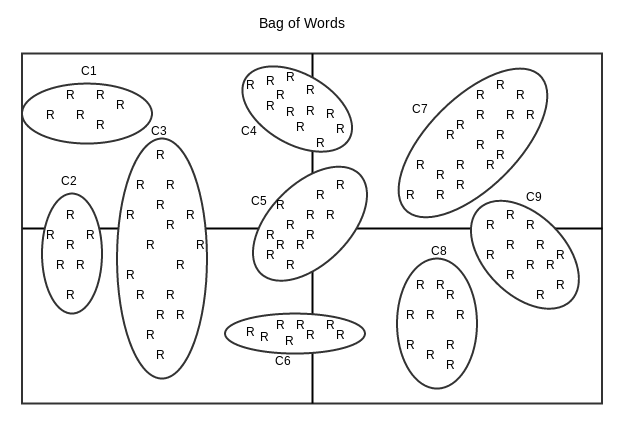
\includegraphics[width=1\textwidth]{Figuras/Diagramas/bow_solo.png}
  		\caption{Construcción del Bag of Words.}
  		\label{algoritmo:fig:bow}
	\end{figure}	

	\subsection{Creación de macro-descriptores}
	\label{algoritmo:crea_macro-descriptores}
	Luego de tener etiquetado cada uno de los \textit{Rayos} $R(x,y)$ con su centroide respectivo, se procede a crear el macro-descriptor de cada uno de los vídeos.	 Esto se realiza creando un histograma de tamaño $K$ para cada uno de las regiones de interés ${ROI}_{i}^{t}$ del vídeo, de tal forma que en este histograma se tenga presente la frecuencia de cada uno de los \textit{clusters} encontrados en la creación del \textit{Bag of Visual Words}. Con esto presente, definimos el descriptor $D_i$ de la región de interés $\text{ROI}_i$ como
	\begin{align}
		\label{algoritmo:eq:hist}
		D_i(k) &= \sum_{(x,y)\in \text{ROI}_i} \delta (R(x,y),k), \quad \forall k,\\
		\label{algoritmo:eq:fun_hist}
		 \delta (R(x,y),k) &= \begin{cases}
		 1 & \mbox{si }R(x,y)~\in~C_k\\
     0 & \text{otro caso}
     \end{cases},
	\end{align}
de tal forma que $\delta(\cdot,\cdot)$ es una función que cuenta los rayos pertenecientes al \textit{cluster} $k$, $C_k$.

	\begin{figure}[bt]
		\centering
		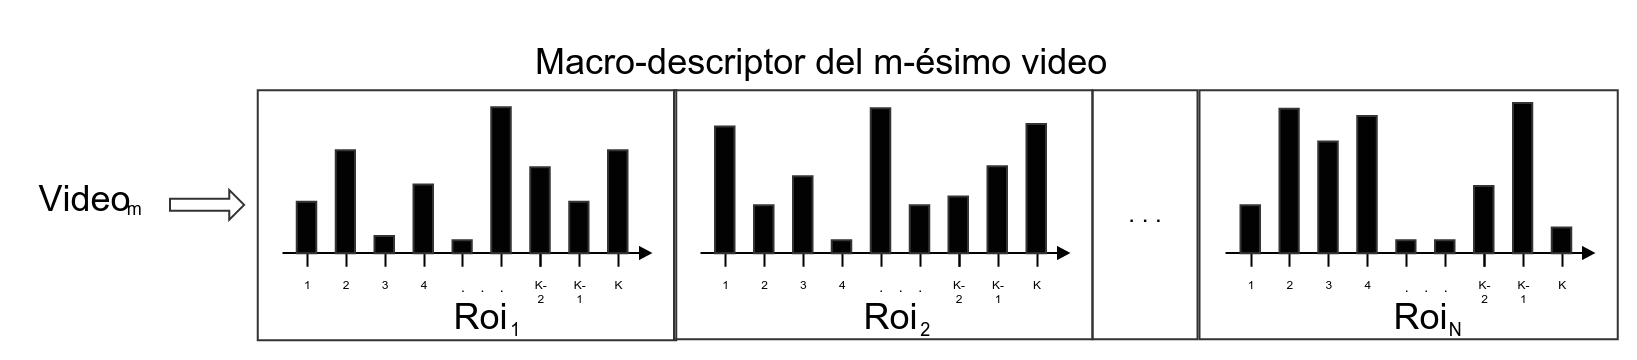
\includegraphics[width=1\textwidth]{Figuras/Diagramas/macro-descriptor.png}
		\caption{Construcción del macro-descriptor.}
		\label{algoritmo:fig:macrodescriptores}
	\end{figure}	

	Luego de obtener dichos descriptores por región, se procede a concatenar cada uno de los histogramas pertenecientes al mismo vídeo de la siguiente forma
	\begin{equation}
		\mathds{D} = \cat_{i = 1}^{I} D_i, \quad \forall i,
	\end{equation}	   
   donde $\cat$ es el operador de concatenación de los vectores $D_i$. Este proceso puede ser visto en la Figura~\ref{algoritmo:fig:macrodescriptores}. El resultado de esta concatenación es el macro-descriptor del vídeo seleccionado.
   


	En el proceso clasificación, no se recalculan los centroides para un nuevo vídeo, ya que, se guarda el modelo que contiene el resultado del \textit{Bag of Visual Words}, y se procede a calcular~(\ref{algoritmo:eq:dist}), para cada uno de los \textit{Rayos} $R(x,y)$ obtenidos en el proceso de extracción de micro-descriptores. Luego de esto al igual que en el proceso de entrenamiento se crea el macro-descriptor con el mismo método.
	
	
\section{Entrenamiento y clasificación}
\label{sec:clasificacion}
El entrenamiento y clasificación es etapa del algoritmo, se dedicada a la segmentación del espacio vectorial formado por los macro-descriptores. Para este proceso se utilizarán las \textit{Support Vector Machines}, explicadas en la Sección~\ref{sec:rec_patrones}. Estás se utilizan para entrenar el modelo que luego es utilizado para clasificar las nuevas entradas de vídeo. 
Para poder probar la efectividad del clasificador se utilizaran técnicas de validación cruzada o $k$\textit{-fold cross-validation} (por sus siglas en inglés). Esta técnica consiste en dividir el conjunto de datos de datos en dos grupos, uno de entrenamiento y uno de prueba, $k$ veces. Esta técnica es utilizada para correr el algoritmo en distintas instancias, y así poder obtener un valor mas real de la precisión. Se mostraran los resultados de esta técnica en la Capítulo~\ref{ch:exp_result}.


		
	\begin{figure}[bt]
		\centering
    		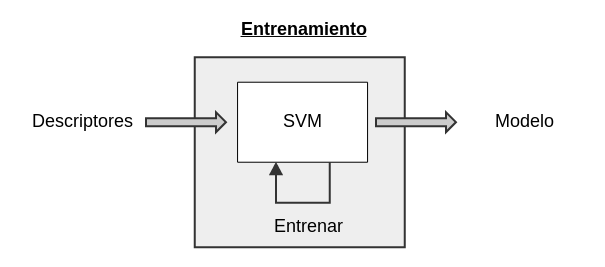
\includegraphics[width=0.7\textwidth]{Figuras/Diagramas/Entrenamiento.png}
  		\caption{Entrenamiento del clasificador.}
  		\label{algoritmo:fig:entrenamiento}
	\end{figure}	
	
	\begin{figure}[bt]
		\centering
    		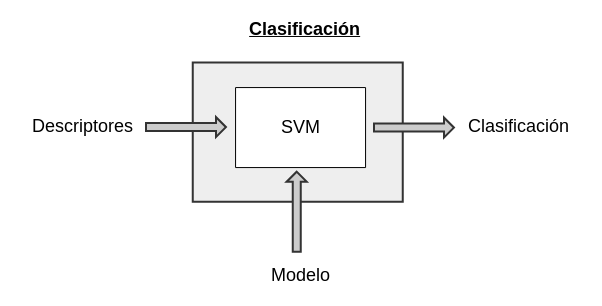
\includegraphics[width=0.7\textwidth]{Figuras/Diagramas/Clasificacion.png}
  		\caption{Clasificador utilizando el modelo creado para clasificar nuevas entradas.}
  		\label{algoritmo:fig:clasificacion}
	\end{figure}	
		
	


	\subsection{Entrenamiento}
	\label{algoritmo:entrenamiento}
		Luego de que el conjunto de datos de entrenamiento pasa por todas las etapas anteriores del algoritmo, se tiene para cada uno de los vídeos un macro-descriptor compuesto por la concatenación de los histogramas de de cada una de las regiones de interés y una etiqueta que indica a que clase pertenecen. Este conjunto de descriptores y las etiquetas son utilizados por las \textit{Support Vector Machines} para la creación de un modelo de clasificación, el que permite poder etiquetar nuevas entradas, este proceso puede ser visto en la Figura~\ref{algoritmo:fig:entrenamiento}.
	
	Las \textit{Support Vector Machines}, son un clasificador de dos clases, entonces es necesario utilizar técnicas que permita realizar la clasificación utilizando muchas clases. Para el caso de esta implementación es necesario poder generar un modelo que permita clasificar las seis expresiones universales. Con este motivo se utiliza la técnica ``\textit{Uno contra uno}'', la cual consiste en generar $C(C-1)/2$ clasificadores, donde cada clase tiene una barrera de decisión asociada a cada una de las demás clases. Esto permite que la región de incertidumbre formada por las barreras de decisión sea mínima.
			
		
	\subsection{Clasificación}
	\label{algoritmo:clasificacion}
		Ya teniendo el modelo resultante de la etapa de entrenamiento, esté es utilizado para la clasificación de nuevas entradas sin etiquetar, esto con la misión de poder asignar una etiqueta al nuevo descriptor, este proceso puede ser visto en la Figura~\ref{algoritmo:fig:clasificacion}. En esta etapa se puede medir cual es la precisión del algoritmo, esta medición sera mayormente abordada en el Capítulo~\ref{ch:exp_result}.
		
	
	
	
	
	

\chapter[Experimentos y resultados]{Experimentos y resultados}
\label{ch:exp_result}

\section{Base de datos MMI}
\label{exp:bdd}
Para poder realizar los experimentos utilizando algoritmo propuesto en el Capítulo~\ref{ch:algoritmo}, se utilizo una base de datos preparada para el reconocimiento facial y de expresiones. Creada por Pantic \etal~\cite{Pantic2005}, MMI es una base de datos multiuso que en esta instancia se utilizo para el reconocimiento de expresiones faciales. Contiene mas de 1000 ejemplos clasificados tanto en imágenes como vídeos; 19 sujetos de prueba; Las edades de los sujetos de prueba varían entre los 19 y los 62 años;  contiene tanto hombres como mujeres, además de tres razas étnicas distintas; Y por último tanto las imágenes como los vídeos están grabados de forma frontal y lateral con respecto al rostro del sujeto. En esta ocasión utilizamos los vídeos grabados de forma frontal, y siendo cada uno de estos etiquetado con una clase distinta para cada expresión facial: Ira~(E1), Asco~(E2), Miedo~(E3), Alegría~(E4), Tristeza~(E5) y Sorpresa~(E6).

\section{Experimentos}
\label{exp:exp}

Para poder probar la efectividad y buen modelado del algoritmo propuesto en el Capítulo~\ref{ch:algoritmo}, se preparo una pila de experimentos, los cuales permitieron realizar una revisión del modelado y precisión de método.
Se prepararon pruebas para cada uno de los pasos del algoritmo, estas pruebas nos permitieron elegir los mejores valores para cada una de las variables a utilizar. Cabe destacar que todos los experimentos realizados sobre el algoritmo, se realizaron en dos instancias de la base de datos MMI, la primera instancia consta de una versión en escala de grises de cada uno de los vídeos, la segunda es una versión a la cual se aplico la técnica LBP descrita en la Sección~\ref{sec:lbp}.

Para la etapa de Extracción de micro-descriptores propuesta en la Sección~\ref{algoritmo:ext_rayos}, se realizaron pruebas que permitieron ver el modelado de los \textit{rayos de flujo} con respecto al movimiento de los pixeles a lo largo de los vídeos, y la elección del tamaño de la Región de soporte $R$ y la Ventana de búsqueda $W$.

En la etapa de Normalización de micro-descriptores, propuesto en la Sección~\ref{algoritmo:normalizacion}, se realizaron pruebas con distintos tamaños de $N$ (Variable utilizada para describir el nuevo tamaño de los \textit{rayos de flujo}) y se realizaron comparaciones con respecto a la Asertividad (\textit{Accuracy} en inglés) de cada valor.

Para la creación de macro-descriptores, propuesta en la Sección~\ref{sec:macro-descriptores}, se prepararon dos experimentos distintos, primero se realizó un estudio del agrupamiento de los \textit{rayos} en el rostro para cada uno de los vídeos con distintos valores $K$, donde $K$ indica la cantidad de grupos de \textit{rayos de flujo} existentes y de que manera se distribuyen en el rostro. El segundo experimento que se realizó fue calcular la Asertividad (\textit{Accuracy} en inglés) para distintos valores de la variable $K$.

Por último en la etapa de entrenamiento y posterior clasificación, explicada en la Sección~\ref{sec:clasificacion}, se realizaron pruebas con los distintos \textit{Kernel} y sus respectivas variables, los cuales son recibidos por SVM para la generación del modelo.


\definecolor{lightgray}{gray}{0.9}
\newlength{\sz}
\setlength{\sz}{2cm}
\begin{table}[t!]
	\centering
	\begin{tabular}{ >{\centering\arraybackslash}m{.2cm}  >{\centering\arraybackslash}m{1.9cm}  >{\centering\arraybackslash}m{1.3cm}  >{\centering\arraybackslash}m{1.5cm}  >{\centering\arraybackslash}m{1.9cm}  >{\centering\arraybackslash}m{1.3cm}  >{\centering\arraybackslash}m{1.5cm}  }
		\hline\noalign{\smallskip}
		& \multicolumn{3}{ c }{Imágenes sin codificación} & \multicolumn{3}{ c }{Imágenes con LBP}\\
		\hline\noalign{\smallskip}
		\raisebox{.8cm}{\rotatebox{90}{\centering\parbox{2cm}{E1--Ira}}} & 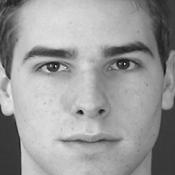
\includegraphics[height=\sz]{Figuras/resultados/E1/E1.png} & 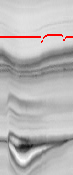
\includegraphics[height=\sz]{Figuras/resultados/E1/E1_YT.png} & 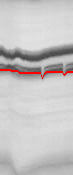
\includegraphics[height=\sz]{Figuras/resultados/E1/E1_XT.png} & 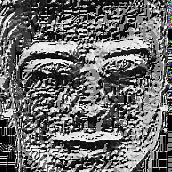
\includegraphics[height=\sz]{Figuras/resultados/E1/E1_LBP.png} & 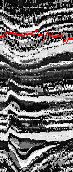
\includegraphics[height=\sz]{Figuras/resultados/E1/E1_LBP_YT.png} & 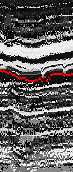
\includegraphics[height=\sz]{Figuras/resultados/E1/E1_LBP_XT.png} \\
		
		\raisebox{.4cm}{\rotatebox{90}{\centering\parbox{2cm}{E2--Asco}}}& 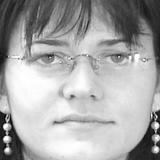
\includegraphics[height=\sz]{Figuras/resultados/E2/E2.png} & 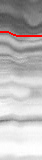
\includegraphics[height=\sz]{Figuras/resultados/E2/E2_YT.png} & 
\includegraphics[height=\sz]{Figuras/resultados/E2/E2_XT.png} & 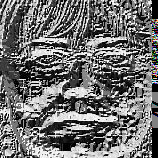
\includegraphics[height=\sz]{Figuras/resultados/E2/E2_LBP.png} & 
\includegraphics[height=\sz]{Figuras/resultados/E2/E2_LBP_YT.png} & 
\includegraphics[height=\sz]{Figuras/resultados/E2/E2_LBP_XT.png} \\
		
		\raisebox{.3cm}{\rotatebox{90}{\centering\parbox{2cm}{E3--Miedo}}}& 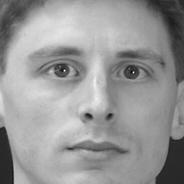
\includegraphics[height=\sz]{Figuras/resultados/E3/E3.png} & 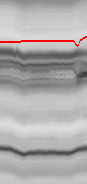
\includegraphics[height=\sz]{Figuras/resultados/E3/E3_YT.png} & 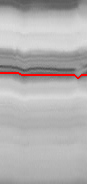
\includegraphics[height=\sz]{Figuras/resultados/E3/E3_XT.png} & 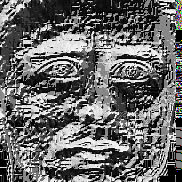
\includegraphics[height=\sz]{Figuras/resultados/E3/E3_LBP.png} & 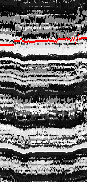
\includegraphics[height=\sz]{Figuras/resultados/E3/E3_LBP_YT.png} & 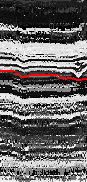
\includegraphics[height=\sz]{Figuras/resultados/E3/E3_LBP_XT.png} \\
		
		\raisebox{.2cm}{\rotatebox{90}{\centering\parbox{2cm}{E4--Alegría}}}& 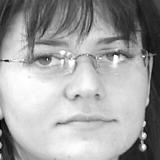
\includegraphics[height=\sz]{Figuras/resultados/E4/E4.png} & 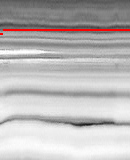
\includegraphics[height=\sz]{Figuras/resultados/E4/E4_YT.png} & 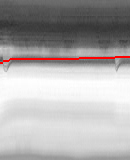
\includegraphics[height=\sz]{Figuras/resultados/E4/E4_XT.png} & 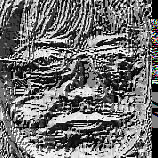
\includegraphics[height=\sz]{Figuras/resultados/E4/E4_LBP.png} & 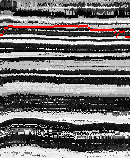
\includegraphics[height=\sz]{Figuras/resultados/E4/E4_LBP_YT.png} & 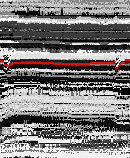
\includegraphics[height=\sz]{Figuras/resultados/E4/E4_LBP_XT.png} \\
		
		\raisebox{0cm}{\rotatebox{90}{\centering\parbox{2cm}{E5--Tristeza}}}& 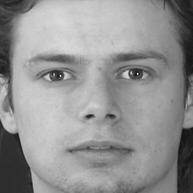
\includegraphics[height=\sz]{Figuras/resultados/E5/E5.png} & 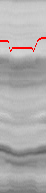
\includegraphics[height=\sz]{Figuras/resultados/E5/E5_YT.png} & 
\includegraphics[height=\sz]{Figuras/resultados/E5/E5_XT.png} & 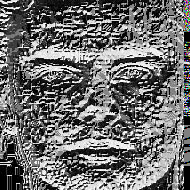
\includegraphics[height=\sz]{Figuras/resultados/E5/E5_LBP.png} & 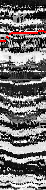
\includegraphics[height=\sz]{Figuras/resultados/E5/E5_LBP_YT.png} & 
\includegraphics[height=\sz]{Figuras/resultados/E5/E5_LBP_XT.png} \\
		
		\raisebox{0cm}{\rotatebox{90}{\centering\parbox{2.1cm}{E6--Sorpresa}}}& 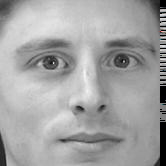
\includegraphics[height=\sz]{Figuras/resultados/E6/E6.png} & 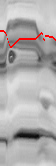
\includegraphics[height=\sz]{Figuras/resultados/E6/E6_YT.png} & 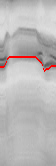
\includegraphics[height=\sz]{Figuras/resultados/E6/E6_XT.png} & 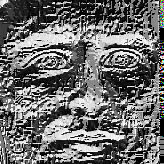
\includegraphics[height=\sz]{Figuras/resultados/E6/E6_LBP.png} & 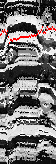
\includegraphics[height=\sz]{Figuras/resultados/E6/E6_LBP_YT.png} & 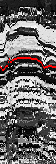
\includegraphics[height=\sz]{Figuras/resultados/E6/E6_LBP_XT.png} \\
		& (a) & (b) & (c) & (d) & (e) & (f) \\

		
	\end{tabular}
	\caption{Tabla comparativa de la extracción de micro-decriptores con vídeos codificados con LBP y sin codificar. Cada fila representa una expresión facial distinta. Las columnas (a) y (d) son el primer cuadro del vídeo, (b) y (e) representan el plano XT, y (c) y (f) representan el plano YT. }
	\label{tabla:comparacion_rayos}
\end{table}


\subsection{Extracción de micro-descriptores}
\label{exp:micro-descriptores}

La extracción de micro-descriptores, etapa propuesta en al Sección~\ref{algoritmo:ext_rayos}, consiste en modelar el movimiento de cada uno de los píxeles a lo largo de todo el vídeo, este modelado es llamado \textit{rayo de flujo}. Para poder extraer un \textit{rayo} se utilizan dos ventanas: la región de soporte y la ventana de búsqueda. Estas regiones permiten calcular a que píxel $(x',y')$ en un tiempo $t+1$ se desplazo el píxel $(x,y)$ en un tiempo $t$. Luego de calcular el movimiento de un píxel de $t$ a $t+1$ se crea un \textit{rayo de soporte}, que es la composición mínima para la creación de los \textit{rayos de flujo}. Para ver en detalle este proceso revisar la Sección~\ref{algoritmo:ext_rayos}.

Para poder evaluar el real modelado de los \textit{rayos} sobre el movimiento de los pixeles, se realizó una extracción de los planos $XT$ y $YT$ del vídeo. El plano $XT$ es una imagen extraída del vídeo en un pixel $(x,y)$, donde cada columna representa un cuadro distinto, cada una de estas son extraídas de sus respectivos cuadros $t$, de tal forma que la columna $t$ del plano $XT$ es la fila $y$ del cuadro $t$ del vídeo. Así mismo el plano $YT$ es otra imagen extraída del vídeo en el mismo pixel $(x,y)$, donde cada columna $t$ de este plano representa un cuadro distinto del vídeo, de tal forma que la columna $t$ del plano $YT$ es la columna $x$ del cuadro $t$ del vídeo. Luego de realizar la extracción de los planos y con la posterior obtención del \textit{rayo de flujo} para el pixel $(x,y)$, fue posible realizar un trazado del movimiento del \textit{rayo} en cada una de sus componentes (En el plano $XT$ se trazo el movimiento de la variable $x$ durante los cuadros del vídeo, por el contrario, en el plano $YT$ se trazó el movimiento de la variable $y$). Ejemplos de estos planos y sus trazos pueden ser vistos en la Tabla~\ref{tabla:comparacion_rayos}, en las columnas (b), (c), (e) y (f).

En general revisando los resultados obtenidos en cada uno de los planos, podemos deducir de forma visual que los \textit{rayos de flujo} modelan de forma aproximada el movimiento de los pixeles. Observando la Tabla~\ref{tabla:comparacion_rayos}, nos dimos cuenta que el modelado de los \textit{rayos} no tiene una mayor variación con respecto a la expresión facial que se esta observando. Al momento de observar las diferencias entre los resultados obtenidos con los vídeos con codificación LBP y sin ésta, pudimos observar que los \textit{rayos} obtenidos en vídeos sin LBP obtenían una mejor aproximación al movimiento real del rayo, este comportamiento puede ser observado al comparar la columna (b) y (e) que representa la extracción en el plano $XT$, o comparando (c) y (f) representantes del plano $YT$ en la Tabla~\ref{tabla:comparacion_rayos}. A su vez se puede observar que las componentes de los \textit{rayos} se comportan mejor al modelar los movimientos verticales (Plano $YT$) que los movimientos horizontales (Plano $XT$), un ejemplo de esto puede ser visto en la expresión (E6), en esta expresión el modelado del movimiento horizontal tiene una aproximación muy baja con respecto a las texturas que se pueden observar en el fondo de la imagen, siendo este un mal modelado de la componente $XT$, por el contrario en la componente del plano $YT$ (columna (c)) se puede observar un modelado casi perfecto con las texturas del fondo de la imagen. Este fenómeno también es visto en otras investigaciones del reconocimiento de expresiones faciales. Ji y Idrissi~\cite{Ji2012} crearon un descriptor espacio temporal que solo utiliza la componente horizontal de los vídeos, ellos se basan en la premisa de que los movimientos significativos del rostro humano tienen una mayor tendencia a ser de forma horizontal que vertical.

\begin{table}[tb]
	\centering
	\begin{tabular}{ >{\centering\arraybackslash}m{2.5cm}  >{\centering\arraybackslash}m{1.2cm}  >{\centering\arraybackslash}m{1.2cm}  >{\centering\arraybackslash}m{1.2cm}  >{\centering\arraybackslash}m{1.2cm}  >{\centering\arraybackslash}m{1.2cm}  >{\centering\arraybackslash}m{1.2cm} }
		\hline
		Codificación & \multicolumn{3}{ c }{XT} & \multicolumn{3}{ c }{YT}\\
		\hline
		& & & & & &\\
		Sin codificación & 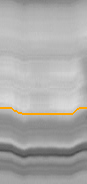
\includegraphics[width=1.2cm]{Figuras/resultados/comparacion_real/no_lbp/XT/extraido.png} & 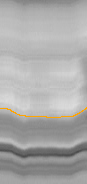
\includegraphics[width=1.2cm]{Figuras/resultados/comparacion_real/no_lbp/XT/pintado.png} & \includegraphics[width=1.2cm]{Figuras/resultados/comparacion_real/no_lbp/XT/superposicion.png} & \includegraphics[width=1.2cm]{Figuras/resultados/comparacion_real/no_lbp/YT/extraido.png} & \includegraphics[width=1.2cm]{Figuras/resultados/comparacion_real/no_lbp/YT/pintado.png} & \includegraphics[width=1.2cm]{Figuras/resultados/comparacion_real/no_lbp/YT/superposicion.png} \\
		
		Codificación LBP & \includegraphics[width=1.2cm]{Figuras/resultados/comparacion_real/lbp/XT/extraido.png} & \includegraphics[width=1.2cm]{Figuras/resultados/comparacion_real/lbp/XT/pintado.png} & \includegraphics[width=1.2cm]{Figuras/resultados/comparacion_real/lbp/XT/superposicion.png} & \includegraphics[width=1.2cm]{Figuras/resultados/comparacion_real/lbp/YT/extraido.png} & \includegraphics[width=1.2cm]{Figuras/resultados/comparacion_real/lbp/YT/pintado.png} & \includegraphics[width=1.2cm]{Figuras/resultados/comparacion_real/lbp/YT/superposicion.png} \\

		& (i) & (ii) & (iii) & (iv) & (v) & (vi)\\

	\end{tabular}
	\caption{Tabla comparativa de el calculo del error de cada plano. (i) y (iv) representan el \textit{rayo} extraído por el algoritmo; (ii) y (v) el \textit{rayo} promedio dibujado por las personas; (iii) y (vi) la superposición de ambos (de color amarillo el extraído y color azul el promedio). }
	\label{tabla:comparacion_errores}
\end{table}


Para poder ratificar las observaciones que hemos podido deducir al contemplar el movimiento a través de los planos, se diseño un experimento que nos permitió calcular un error aproximado del modelado de los \textit{rayos de flujo}. Este experimento consistió en pedir a distintas personas que dibujaran el \textit{rayo de flujo} sobre cada plano, para esto utilizaron la herramienta de dibujo paint de Windows. En general se pidió a cada una de las personas que dibujaran como creían ellos que se movía el pixel inicial a lo largo de las texturas representadas en el plano. Luego de esta etapa se procedió a extraer cada una de las componentes de los \textit{rayos} dibujados a mano, con esto se logro calcular un promedio de los trazos de las personas. Este \textit{rayo} promedio es comparado con el extraído por el algoritmo, de tal forma que se puede calcular el error para cada componente y un error general. Este proceso puede ser visualizado en la Tabla~\ref{tabla:comparacion_errores}, donde las columnas (iii) y (iv), representan de forma visual como se superpone un \textit{rayo} sobre otro. El error es obtenido calculando la desviación estándar entre ambas componentes. 

\pgfplotstableset{
  franjas/.style={
    columns/errorG/.style={
      column name=Error,
      precision=1
    },
    every even row/.style={
      before row={\rowcolor{#1}}
    },
    every head row/.style={
      before row=\hline\noalign{\smallskip},after row=\hline
    },
    every last row/.style={
      after row=\hline
    }
  },
  franjas/.default={gray!50},
  tablita/.style={
    columns={rs, ws, errorXT, errorYT, errorG},
    columns/rs/.style={
      column name=$RS$,
    },
    columns/ws/.style={
      column name=$WS$,
    },
    columns/errorXT/.style={
      column name=Error $XT$,
      precision=1
    },
    columns/errorYT/.style={
      column name=Error $YT$,
      precision=1
    },
    franjas,
  },
  tablaK/.style={
  	columns={N, K, Accuracy},
  	columns/N/.style={
  		column name=$N$,
  	},
  	columns/K/.style={
  		column name=$K$,
  	},
  	columns/Accuracy/.style={
  		column name=Accuracy,
  		precision=1,
  		postproc cell content/.append style={
  			/pgfplots/table/@cell content/.add={}{\,\%}
  		}
  	},
  	franjas,
  },
  tablaN/.style={
  	columns={RS, WS, N, Accuracy},
  	columns/RS/.style={
  		column name=$RS$,
  	},
  	columns/WS/.style={
  		column name=$WS$,
  	},
  	columns/N/.style={
  		column name=$N$,
  	},
  	columns/Accuracy/.style={
  		column name=Accuracy,
  		precision=1,
  		postproc cell content/.append style={
  			/pgfplots/table/@cell content/.add={}{\,\%}
  		}
  	},
  	franjas,
  },
  tablaSVMresultsRBF/.style={
  	columns={Gamma,C-value,Accuracy},
  	columns/Gamma/.style={
  		column name=$Gamma$,
  		precision=3
  	},
  	columns/C-value/.style={
  		column name=$C-value$,
  		precision=3
  	},
  	columns/Accuracy/.style={
  		column name=$Accuracy$,
  		precision=1,
  		postproc cell content/.append style={
  			/pgfplots/table/@cell content/.add={}{\,\%}
  		}
  	},
  	franjas,
  },
  tablaSVMresultsLineal/.style={
  	columns={C-value,Accuracy},
  	columns/C-value/.style={
  		column name=$C-value$,
  		precision=3
  	},
  	columns/Accuracy/.style={
  		column name=$Accuracy$,
  		precision=1,
  		postproc cell content/.append style={
  			/pgfplots/table/@cell content/.add={}{\,\%}
  		}
  	},
  	franjas,
  },
  tablaSVMresultsPoly/.style={
  	columns={Degree,Gamma,C-value,Accuracy},
  	columns/Degree/.style={
  		column name=$Degree$,
  	},
  	columns/Gamma/.style={
  		column name=$Gamma$,
  		precision=3
  	},
  	columns/C-value/.style={
  		column name=$C-value$,
  		precision=3
  	},
  	columns/Accuracy/.style={
  		column name=$Accuracy$,
  		precision=1,
  		postproc cell content/.append style={
  			/pgfplots/table/@cell content/.add={}{\,\%}
  		}
  	},
  	franjas,
  },
  tablaSVMresults/.style={
  	columns={RS,WS,N,K,Accuracy},
  	columns/RS/.style={
  		column name=$RS$,
  	},
  	columns/WS/.style={
  		column name=$WS$,
  	},
  	columns/N/.style={
  		column name=$N$,
  	},
  	columns/K/.style={
  		column name=$K$,
  	},
  	columns/Accuracy/.style={
  		column name=$Accuracy$,
  		precision=1,
  		postproc cell content/.append style={
  			/pgfplots/table/@cell content/.add={}{\,\%}
  		}
  	},
  	franjas,
  },
}

\begin{table}[tb]
	\centering
	\pgfplotstabletypeset[tablita]{Datos/comparacion_NO_LBP.dat}
	\caption{Tabla comparativa de los errores encontrados en los planos $XT$, $YT$ y error general, al calcular los \textit{rayos} con distintos tamaños de ventanas. Sin codificación LBP.}
	\label{tabla:error_no_lbp}
\end{table}

\begin{table}[tb]
	\centering
	\pgfplotstabletypeset[tablita]{Datos/comparacion_LBP.dat}
	\caption{Tabla comparativa de los errores encontrados en los planos $XT$, $YT$ y error general, al calcular los \textit{rayos} con distintos tamaños de ventanas. Con codificación LBP.}
	\label{tabla:error_lbp}
\end{table}

Decidimos utilizar esta métrica de comparación para visualizar cómo se comportan los \textit{rayos} con respecto al tamaño de las ventanas utilizadas, En las Tablas~\ref{tabla:error_no_lbp}~y~\ref{tabla:error_lbp} se puede ver reflejados los cálculos resultantes del error en ambos planos y el error general calculado como el promedio entre ambos errores, utilizando distintos tamaños de ventanas. Con estos resultados logramos darnos cuenta que la idea planteada sobre las diferencias del modelado vertical y horizontal estaba en lo cierto, en ambas tablas podemos ver que el error obtenido en el plano $XT$ es mucho menor al obtenido en $YT$. Además en general los errores disminuyen a medida que se aumenta el tamaño de las ventanas $RS$ y $WS$, esto es debido a que mientras mas grande sea la región de soporte, menos probabilidad existe de encontrar otra textura igual en la imagen, por lo cual la probabilidad de encontrar en el siguiente cuadro el movimiento de la misma textura es mucho mas alta.

\begin{figure}[t]
	\begin{subfigure}{1.0\textwidth}
		\centering
		\includegraphics[width=1\textwidth]{Figuras/resultados/videos_sinteticos/v1.png}
		\caption{Vídeo sintético simple sin texturas}
		\label{exp:fig:vs1}
	\end{subfigure}
	
	\begin{subfigure}{1.0\textwidth}
		\centering
		\includegraphics[width=1\textwidth]{Figuras/resultados/videos_sinteticos/v2.png}
		\caption{Vídeo sintético simple con texturas}
		\label{exp:fig:vs2}
	\end{subfigure}
	
	\begin{subfigure}{1.0\textwidth}
		\centering
		\includegraphics[width=1\textwidth]{Figuras/resultados/videos_sinteticos/v3.png}
		\caption{Vídeo sintético con texturas.}
		\label{exp:fig:vs3}
	\end{subfigure}
	\caption{Cortes de vídeos sintéticos, en los cuales se describe el movimiento de ciertos pixeles a los largo del tiempo.} 
	\label{exp:fig:vs}
\end{figure}

Luego de obtener resultados satisfactorios con el modelado de los \textit{rayos de flujo}, decidimos probar si la teoría de extracción de estos podía ser aplicada a otros vídeos y otras texturas, por lo que preparamos un conjunto de vídeos sintéticos, los cuales describían movimientos predecibles al ojo humano. En estos vídeos se represento el movimiento de regiones cuadradas con y sin textura, y también se genero un vídeo que permitió examinar que sucede con los rayos si existen dos movimientos distintos.

Luego de realizar la extracción de \textit{rayos de flujo} a los vídeos generados sintéticamente, observamos dos fenómenos. Los rayos pueden modelar el movimiento de los píxeles a los largo del tiempo, esto puede ser visto en la Figura~\ref{exp:fig:vs}, en la cual se ven cortes de distintos cuadros de los vídeos y como se mueven los píxeles escogidos, estos pixeles son representados con cuadros de color a lo largo del vídeo. También descubrimos que el modelado de los \textit{rayos} tiene un comportamiento mas estable cuando existen texturas en las zonas que se están analizando, como se puede ver en las Figuras~\ref{exp:fig:vs2}~y~\ref{exp:fig:vs3}, los píxeles internos del cuadrado siguen durante todo el movimiento en la misma posición del cuadrado, no así en la Figura~\ref{exp:fig:vs1}, en la cual los pixeles que están dentro del cuadrado tienden a juntarse en un punto a medida que el cuadrado se va desplazando. 

En general, por lo que pudimos apreciar en el desarrollo de todos estos experimentos, el comportamiento de los \textit{rayos} depende de dos componentes claves para conseguir un buen modelado, primero una elección inteligente del tamaño de las ventanas $RS$ y $WS$, esto debido a que una ventana más grande disminuyes las probabilidades de error a la hora de elegir el movimiento del pixel, pero a su vez aumenta el costo computacional del algoritmo, debido a que se deben realizar mas cálculos a la hora de la elección del movimiento; segundo, otra componente clave es el nivel de detalle de la textura abarcada por las ventanas, esto debido a que una textura plana puede ser fácilmente confundida con otra textura plana similar, a su vez una textura con detalle permite que el modelado sea más real con respecto a los reales movimientos del rostro humano. 

\subsection{ Normalización de micro-descriptores }

Luego de concretar la extracción de los micro-descriptores, Se procedió a realizar una normalización de los \textit{rayos de flujo}, ésta consistió en poder realizar una reducción o ampliación de los rayos, esto con el fin de que todos los micro-descriptores tengan el mismo largo $N$, ésto nos permitió tener a todos los \textit{rayos} en el mismo espacio vectorial. Para detalles sobre esta etapa revisar la Sección~\ref{algoritmo:normalizacion}.
\begin{table}[b]
	\centering
	\pgfplotstabletypeset[tablaN]{Figuras/resultados/Normalizacion/Accuracy_n.dat}
	\caption{Tabla comparativa de la Asertividad o \textit{Accuracy} (en ingles) obtenido utilizando distintos valores de $N$ y distintos tamaños de las ventanas.}
	\label{tabla:accuracy_N}
\end{table}

Para poder evaluar que valores de la variable $N$ escoger al momento de realizar la normalización, se decidió realizar una comparación entre el valor de la variable $N$ y la asertividad o \textit{Accuracy} reconociendo las expresiones faciales. Estos resultados pueden ser vistos en la Tabla~\ref{tabla:accuracy_N}, para obtener resultados se utilizaron valores de las ventanas $RS$ y $WS$ estudiados en la Sección~\ref{exp:micro-descriptores}. 

Observando los resultados logramos deducir que no existe una gran variación en el \textit{Accuracy} con respecto a los valores de la normalización. En general observamos que el comportamiento de la asertividad no tenia una dependencia muy directa del tamaño de la normalización, esto debido a que este procedimiento lo único que hace es realizar proyección lineal del espacio vectorial sobre un nuevo espacio parametrizado por la variable $N$, visto desde la parte matemática, este procedimiento además de ayudar a poder comparar vectores de distintas dimensiones, permitió realizar una transformación de cada uno de estos \textit{rayos} a un espacio vectorial común para su posterior agrupamiento. 



\subsection{ Creación de macro-descriptores }

La creación de los macro-descriptores es la etapa final de la extracción de características de los vídeos, se utilizó la técnica \textit{Bag of visual words} analizada en la Sección~\ref{sec:bag_of_words}, para obtener un diccionario que permita representar el espacio vectorial a analizar, en el caso de nuestra implementación es necesario obtener un conjunto de \textit{rayos de flujo} representativos del espacio, este conjunto es llamado vocabulario, y en el se encuentran todas las posibles palabras que pueden existir en el universo formado por los datos de entradas. Para poder obtener este vocabulario sobre nuestros micro-descriptores, se utilizó la técnica de agrupamiento no supervisada $k$-means analizada en la Seccion~\ref{sec:k-means}, la cual recibe como entrada un grupo de vectores (\textit{rayos de flujo}) y la cantidad $K$ de grupos a formar, con esto calcula cada uno de los vectores o \textit{rayos} representantes, los cuales son el vocabulario utilizado por el \textit{Bag of visual words}. Luego de obtener este vocabulario, se procede a construir los macro-descriptores de cada vídeo, calculando un histograma de tamaño $K$, el cual es la representación de la frecuencia de asociación de cada \textit{rayo} con su respectivo \textit{cluster} $k$. Para mas detalles de esta etapa revisar la Sección~\ref{sec:macro-descriptores}. Con esto logramos deducir que la variable $K$, es de suma importancia para el algoritmo, esto debido a que la construcción de los descriptores finales de cada vídeo dependen del valor asignado a esta variable.

\newlength{\st}
\setlength{\st}{1.5cm}
\setlength{\sz}{1.6cm}
\begin{table}[tb]
	\centering
	\begin{tabular}{ >{\centering\arraybackslash}m{.5cm}  >{\centering\arraybackslash}m{\st}  >{\centering\arraybackslash}m{\st}  >{\centering\arraybackslash}m{\st}  >{\centering\arraybackslash}m{\st}  >{\centering\arraybackslash}m{\st}  >{\centering\arraybackslash}m{\st}  }
		\hline\noalign{\smallskip}
		$K$ & Ira & Asco & Miedo & Alegría & Tristeza & Sorpresa\\
		\hline\noalign{\smallskip}
		10 & \includegraphics[height=\sz]{Figuras/resultados/clustering/k=10/E1_ec.png} & \includegraphics[height=\sz]{Figuras/resultados/clustering/k=10/E2_ec.png} & \includegraphics[height=\sz]{Figuras/resultados/clustering/k=10/E3_ec.png} & \includegraphics[height=\sz]{Figuras/resultados/clustering/k=10/E4_ec.png} & \includegraphics[height=\sz]{Figuras/resultados/clustering/k=10/E5_ec.png} & \includegraphics[height=\sz]{Figuras/resultados/clustering/k=10/E6_ec.png} \\
		
		50 & \includegraphics[height=\sz]{Figuras/resultados/clustering/k=50/E1_ec.png} & \includegraphics[height=\sz]{Figuras/resultados/clustering/k=50/E2_ec.png} & \includegraphics[height=\sz]{Figuras/resultados/clustering/k=50/E3_ec.png} & \includegraphics[height=\sz]{Figuras/resultados/clustering/k=50/E4_ec.png} & \includegraphics[height=\sz]{Figuras/resultados/clustering/k=50/E5_ec.png} & \includegraphics[height=\sz]{Figuras/resultados/clustering/k=50/E6_ec.png} \\
		
		100 & \includegraphics[height=\sz]{Figuras/resultados/clustering/k=100/E1_ec.png} & \includegraphics[height=\sz]{Figuras/resultados/clustering/k=100/E2_ec.png} & \includegraphics[height=\sz]{Figuras/resultados/clustering/k=100/E3_ec.png} & \includegraphics[height=\sz]{Figuras/resultados/clustering/k=100/E4_ec.png} & \includegraphics[height=\sz]{Figuras/resultados/clustering/k=100/E5_ec.png} & \includegraphics[height=\sz]{Figuras/resultados/clustering/k=100/E6_ec.png} \\
		
		500 & \includegraphics[height=\sz]{Figuras/resultados/clustering/k=500/E1_ec.png} & \includegraphics[height=\sz]{Figuras/resultados/clustering/k=500/E2_ec.png} & \includegraphics[height=\sz]{Figuras/resultados/clustering/k=500/E3_ec.png} & \includegraphics[height=\sz]{Figuras/resultados/clustering/k=500/E4_ec.png} & \includegraphics[height=\sz]{Figuras/resultados/clustering/k=500/E5_ec.png} & \includegraphics[height=\sz]{Figuras/resultados/clustering/k=500/E6_ec.png} \\
		
		1000 & \includegraphics[height=\sz]{Figuras/resultados/clustering/k=1000/E1_ec.png} & \includegraphics[height=\sz]{Figuras/resultados/clustering/k=1000/E2_ec.png} & \includegraphics[height=\sz]{Figuras/resultados/clustering/k=1000/E3_ec.png} & \includegraphics[height=\sz]{Figuras/resultados/clustering/k=1000/E4_ec.png} & \includegraphics[height=\sz]{Figuras/resultados/clustering/k=1000/E5_ec.png} & \includegraphics[height=\sz]{Figuras/resultados/clustering/k=1000/E6_ec.png} \\
		
		& (E1) & (E2) & (E3) & (E4) & (E5) & (E6) \\
	\end{tabular}
	\caption{Tabla comparativa de la cantidad de \textit{cluster} utilizados y su representación en las distintas expresiones faciales. Las imágenes fueron construidas en escala de grises, los colores mas cercanos al blanco representan mayor cantidad de \textit{rayos} agrupados en ese conjunto. }
	\label{tabla:comparacion_clusters} 
\end{table}	

\begin{table}[tb]
	\centering
	\pgfplotstabletypeset[tablaK]{Figuras/resultados/clustering/Accuracy_k.dat}
	\caption{Tabla comparativa de la Asertividad o \textit{Accuracy} (en ingles) obtenido utilizando distintos valores de $K$.}
	\label{tabla:accuracy_K}
\end{table}

Para poder evaluar si esta técnica realizó un modelado exitoso preparamos dos experimentos, el primero consistió en poder realizar una evaluación visual del movimiento de los grupos o \textit{clusters} de \textit{rayos}, siendo estos representados sobre el rostro que fue analizado. En general sabemos por la extracción de \textit{rayos de flujo}, que cada uno de estos tiene asociada una posición inicial dentro del rostro analizado, con lo cual se procedió a crear imágenes en escala de grises, las cuales representan los \textit{clusters} dentro del vídeo. Algunos ejemplos pueden ser vistos en la Tabla~\ref{tabla:comparacion_clusters}. 

Las imágenes fueron construidas calculando y ordenando los $P$ grupos con mayor frecuencia ( 0 <\ $P$ <\ 255 y $P \leq K$ ), cada grupo $p$ fue asignado a un valor en la escala de grises, a los grupos que obtuvieron una mayor frecuencia de aparición les fueron asignado valores mas cercanos a $255$ (Color blanco), del mismo modo los \textit{clusters} con menor frecuencia obtienen valores mas cercanos a $0$ (Color negro), a su vez todos los demás grupos que quedaron fuera de la selección inicial reciben el valor $0$. Esto debido a que los \textit{cluster} con menor frecuencia pueden ser catalogados como \textit{rayos} ruidosos, y que no aportan información al sistema.

Observando las imágenes obtenidas y representadas en la Tabla~\ref{tabla:comparacion_clusters}, logramos percatarnos que existe una gran segmentación de las regiones más importantes del rostro (Ojos, cejas, nariz y boca). A medida que la variable $K$ aumenta, logramos visualizar de mejor manera las regiones de interés. El ejemplo mas característico puede ser visualizado en la expresión de sorpresa (E6), cuando $K$ tomó el valor 10, en (E6) observamos una tendencia de los \textit{clusters} a agruparse en las regiones importantes, conforme fue aumentando el valor de $K$, la imagen del rostro se fue volviendo mas nítida llegando a detectar visualmente de forma muy directa las partes importantes del rostro (véase la secuencia de imágenes de (E6) con distintos valores $K$), así mismo esto paso con el general de los vídeos utilizados en los experimentos. También logramos deducir que visualmente no existe una dependencia entre la expresión facial que se quiso representar y las regiones del rostro más nítidas.

Cabe destacar que por las observaciones realizadas, es de vital importancia una elección inteligente de la cantidad de grupos a crear, esto debido a que un valor muy pequeño puede hacer que los conjuntos encontrados estén muy poco segmentados (Ver k = 10 en la Tabla~\ref{tabla:comparacion_clusters}), por el contrario un valor muy alto puede provocar una sobre segmentación de los \textit{cluster}, de tal forma que los \textit{rayos} estén tan segmentados que los clasificadores no puedan encontrar patrones en los macro-descriptores de la misma expresión.

El segundo experimento consistió en buscar de forma mas empírica un valor que permita la creación de un buen modelo de clasificación a la hora de etiquetar nuevas expresiones entrantes. Para esto se realizó una comparación de distintos valores $K$ y su asertividad a la hora de clasificar. Estos resultados son expuestos en la Tabla~\ref{tabla:accuracy_K}, y fueron obtenidos al utilizar los mejores valores resultantes en las variables analizadas en las secciones anteriores de este capítulo, los datos obtenidos son bastante pobres a pesar de los cambios de la variable $K$, esto puede ser debido a un mal agrupamiento por parte del algoritmo. Es de vital importancia mencionar que los algoritmos de \textit{clustering} son muy sensibles a las semillas ingresadas como puntos iniciales, para estos experimentos utilizamos un algoritmo de elección inteligente de las semillas, este método esta basado en las investigaciones de Arthur y Vassilvitskii~\cite{Arthur2007}, el cual esta implementado en la librería OpenCV.

En general, luego de observar los resultados de los experimentos expuestos, se pudo visualizar una necesidad de seguir profundizando en el tema de como construir los macro-descriptores, proponemos realizar investigaciones sobre los distintos algoritmos que se pueden utilizar a la hora de agrupar, cuales medidas de distancia permiten un mejor agrupamiento de los \textit{rayos}, buscar como inicializar de mejor manera las semillas. Por otra parte revisando los resultados obtenidos al realizar el mapeo de los \textit{clusters} en el rostro surgieron dudas sobre que es lo que pasaría si la extracción de rayos se realizara solo sobre las regiones importantes del rostro, esto ¿daría pie a un agrupamiento mas localizado sobre las regiones que realmente nos interesa saber su movimiento?. 


\subsection{ Entrenamiento y clasificación }


\begin{table}[tb]
	\centering
	\pgfplotstabletypeset[tablaSVMresultsRBF]{Datos/rbf_10.csv}
	\caption{Mejores resultados obtenidos por el Kernel RBF.}
	\label{tabla:svm_rbf}
\end{table}
\begin{table}[tb]
	\centering
	\pgfplotstabletypeset[tablaSVMresultsLineal]{Datos/lineal_10.csv}
	\caption{Mejores resultados obtenidos por el Kernel Lineal.}
	\label{tabla:svm_lineal}
\end{table}
\begin{table}[tb]
	\centering
	\pgfplotstabletypeset[tablaSVMresultsPoly]{Datos/poly_10.csv}
	\caption{Mejores resultados obtenidos por el Kernel Polinomial.}
	\label{tabla:svm_poly}
\end{table}

El entrenamiento y clasificación es de vital importancia, debido a que en esta etapa es cuando se genera el modelo que permite clasificar las nuevas expresiones entrantes. Este modulo puede ser dividido en dos partes, primero el entrenamiento, el cual es el encargado de encontrar un modelo que permita clasificar de la mejor forma las nuevas entradas; segundo la clasificación, etapa encargada de etiqueta con alguna expresión las nuevas entradas, esta etiqueta es asignada dependiendo del modelo entrenado en la fase anterior. También en esta etapa se realiza el calculo de la asertividad o \textit{Accuracy} (Por sus siglas en ingles) del algoritmo. Para obtener un calculo mas real del modelo generado se utilizó la técnica de $k$-fold cross-validation, la cual en simples palabras consiste en separar los datos de forma aleatoria en dos grupos (Entrenamiento y pruebas), realizando esta separación $k$ veces y para cada una de estas separaciones obteniendo un \textit{Accuracy} el cual es el promediado de todas separaciones, este promedio es el promedio que se utiliza como medida de comparación. Para todos los experimentos expuestos en esta Sección se utilizo un 10-fold cross validación y SVM. Para mayores detalles de esta etapa, revisar la Sección~\ref{sec:clasificacion}.

Como se explico en la Sección~\ref{sec:svm}, SVM trata de encontrar una recta que permita separar a los dos grupos datos dentro de un mismo espacio vectorial, en el general de los casos reales no existe una recta que permita separar de forma efectiva ambas clases, por esto SVM hace uso de las técnicas de Kernel, en simples palabras estas técnicas permiten realizar transformación lineales de los espacios vectoriales, con lo cual se puede realizar la búsqueda de un hiper-plano que logre segmentar ambas clases y minimice el error. Debido a esto realizamos un experimento que permita encontrar de forma empírica cual de los Kernel y valores de sus respectivas variables maximicen el \textit{Accuracy}, Los Kernels utilizados están implementados en la librería en Opencv la cual se basa LibSVM creada por Chang~y~Lin~\cite{Chang2011} para obtener resultados de SVM.


Como se puede observar en las Tablas~\ref{tabla:svm_rbf},~\ref{tabla:svm_lineal}~y~\ref{tabla:svm_poly}, se obtuvieron resultados muy bajos, en general, los mejores \textit{Accuracy} fueron obtenidos utilizando el Kernel RBF, el cual permite realizar una transformación lineal, donde una recta en el espacio del Kernel puede ser representada por una circunferencia en el plano real de los datos. Revisando los valores de las variables ($\gamma$, \textit{Degree} y $C$-value), observamos que no existe una segmentación clara sobre que valores deben adquirir estas variables para obtener mejores resultado a la hora de entrenar el modelo. En la Sección~\ref{sec:svm}, nombramos distintos kernels que podrían ser utilizados para el problema de clasificación, entre ellos \textit{Histogram Intersection}, el cual tiene una gran efectividad a la hora de generar un modelo de vectores representantes de histogramas, este kernel no esta incluido en la implementación de SVM en la librería OpenCV. Por lo cual es importante buscar alguna implementan de SVM que tenga incluido este kernel.

\begin{table}[tb]
	\centering
	\pgfplotstabletypeset[tablaSVMresults]{Datos/resultados.dat}
	\caption{Resultados obtenidos utilizando las mejores variables obtenidas en el proceso de experimentos.}
	\label{tabla:exp:accuracy}
\end{table}


Por ultimo como experimento final decidimos realizar una comparación del \textit{Accuracy} obtenido con mejores valores de las variables del algoritmo ($RS$, $WS$, $N$, $K$). Esta comparación puede ser visualizada en la Tabla~\ref{tabla:exp:accuracy}.

En general y al igual que en la mayoría de los experimentos de obtención de \textit{Accuracy}, se obtuvieron resultados muy pobres, esto puede ser debido a una mala aproximacion de los valores de las variables de los kernels, o que los kernels que se utilizan no permiten realizar un mapeo exitoso del espacio vectorial observado. Otro posible problema puede ser el tamaño de los conjuntos de entrenamiento y prueba utilizados por el $k$-fold cross validation, debido a que para todos los experimentos se utilizo un 50\% de los videos para el entrenamiento, por lo cual puede existir una necesidad del clasificador por tener mas datos de entrenamiento, para así poder obtener un mejor modelo de clasificación.


\chapter[Conclusión]{Conclusión}
\label{ch:conclusion}

%
% genero más documento de forma aleatoria
\blinddocument

% Genero toda las referencias para demostrar el uso de la bibliografía
% No es necesario que utilice este comando en su documento.
\nocite{*}

% incluya otros archivos según su necesidad
% \input{archivo}


% Iniciamos el resto de secciones adicionales al contenido: referencias y apendices
\backmatter


% Bibliografía
% referencias.bib es el archivo con la base de datos bibliografica
% se recomienda utilizar un manejador de referencias: Jabref (jabref.sourceforge.net)
% El estilo por defecto es IEEE Transactions
\bibliographystyle{ieeetr}
% Acá puede incluir uno más archivos de referencia
\bibliography{referencias}


% Simbología y glosario
% Utilice un paquete para generar símbolos y glosarios.
% Por ejemplo: nomencl (http://texdoc.net/pkg/nomencl)


% Anexos
%\appendix

% Aca se incluyen los archivos con el texto de los anexos
% Por ejemplo, anexo.tex
%\chapter{Primer anexo}
\label{ch:anexo-a}

%\blindtext[5]


\chapter{Segundo anexo}
\label{ch:anexo-b}


%\blindtext[10]



% puede incluir más archivos de anexos
% \input{anexo-dos}

\end{document}
% that's all folks